% mnras_template.tex
%
% LaTeX template for creating an MNRAS paper
%
% v3.0 released 14 May 2015
% (version numbers match those of mnras.cls)
%
% Copyright (C) Royal Astronomical Society 2015
% Authors:
% Keith T. Smith (Royal Astronomical Society)

% Change log
%
% v3.0 May 2015
%    Renamed to match the new package name
%    Version number matches mnras.cls
%    A few minor tweaks to wording
% v1.0 September 2013
%    Beta testing only - never publicly released
%    First version: a simple (ish) template for creating an MNRAS paper

%%%%%%%%%%%%%%%%%%%%%%%%%%%%%%%%%%%%%%%%%%%%%%%%%%
% Basic setup. Most papers should leave these options alone.
\documentclass[a4paper,fleqn,usenatbib]{mnras}

% MNRAS is set in Times font. If you don't have this installed (most LaTeX
% installations will be fine) or prefer the old Computer Modern fonts, comment
% out the following line
\usepackage{newtxtext,newtxmath}

% Use vector fonts, so it zooms properly in on-screen viewing software
% Don't change these lines unless you know what you are doing
\usepackage[T1]{fontenc}
\usepackage{ae,aecompl}


%%%%% AUTHORS - PLACE YOUR OWN PACKAGES HERE %%%%%

% Only include extra packages if you really need them. Common packages are:
\usepackage{graphicx}	% Including figure files
\usepackage{amsmath}	% Advanced maths commands
\usepackage{amssymb}	% Extra maths symbols

% \usepackage[flushleft, referable]{threeparttablex} % Adding notes under tables
\usepackage[version=4]{mhchem} 	% typeset chemistry symbols
\usepackage{array} % For wrapping text in cell in tables with multicolumntype
% \usepackage{pdflscape} % for landscape pages
\usepackage{color,soul} % highlighting
\DeclareRobustCommand{\removed}[1]{{\sethlcolor{red}\hl{#1}}}
\DeclareRobustCommand{\added}[1]{{\sethlcolor{green}\hl{#1}}}


\soulregister\cite7
\soulregister\citep7
\soulregister\citet7
\soulregister\citealt7
\soulregister\ref7
\soulregister\textbf7
\soulregister\ 7
\soulregister\ion7
\soulregister\subsubsection7
\soulregister\subsubsection1



% *****************************************************************
% THis is my setting to avoid a particular LaTeX error due to links running
% onto new pages.
\hypersetup{draft}
% *****************************************************************


%%%%%%%%%%%%%%%%%%%%%%%%%%%%%%%%%%%%%%%%%%%%%%%%%%

%%%%% AUTHORS - PLACE YOUR OWN COMMANDS HERE %%%%%

% Please keep new commands to a minimum, and use \newcommand not \def to avoid
% overwriting existing commands. Example:
%\newcommand{\pcm}{\,cm$^{-2}$}	% per cm-squared
\defcitealias{Thomas2010}{TMJ} % TMJ alias
\newcolumntype{L}[1]{>{\raggedright\let\newline\\\arraybackslash\hspace{0pt}}m{#1}} % Multi-column entries in tables with text wrapping 
\newcommand{\bracket}[1]{[#1]} % to be able to use [] in arguments


%%%%%%%%%%%%%%%%%%%%%%%%%%%%%%%%%%%%%%%%%%%%%%%%%%

%%%%%%%%%%%%%%%%%%% TITLE PAGE %%%%%%%%%%%%%%%%%%%

% Title of the paper, and the short title which is used in the headers.
% Keep the title short and informative.
\title[IFS Study of Low-power Radio Galaxies]{An Integral-field
  Spectroscopic Study of Low-power Radio Galaxies}

% The list of authors, and the short list which is used in the headers.
% If you need two or more lines of authors, add an extra line using \newauthor
\author[J. Warren et al.]{
  Joshua Warren,$^{1}$\thanks{Contact e-mail:
    \href{mailto:warrenj@gmx.com}{warrenj@gmx.com}}
%Joshua Warren,$^{1}$\thanks{Contact e-mail: \href{mailto:joshua.warren@physics.ox.ac.uk}{joshua.warren@physics.ox.ac.uk}}
  Martin Bureau,$^{1,2}$ Bernd Hasemann,$^{3}$ \added{Ilaria Ruffa,$^{4}$} Isabella
  Prandoni,$^{4}$ \newauthor Francesco Santoro,$^{4}$ Robert
  Laing,$^{4}$ Paola Parma,$^{4}$ \added{Rosita Paladino,$^{4}$} Hans de Ruiter,$^{4}$ \newauthor
  Arturo Mignano$^{4}$ and \added{Timothy Davis$^{5}$}
  \\
  $^{1}$Sub-department of Astrophysics, Department of Physics,
  University of Oxford, Denys Wilkinson Building, Keble Road, Oxford
  OX1 3RH, UK\\
  $^{2}$Yonsei Frontier Lab and Department of Astronomy, Yonsei
  University, 50 Yonsei-ro, Seodaemun-gu, Seoul 03722, Republic of
  Korea\\
  $^{3}$European Southern Observatory, Karl-Schwarzschild-Str.\ 2,
  85748 Garching b.\ M{\"u}nchen, Germany\\
  $^{4}$INAF - Istituto di Radioastronomia, Via P.\ Gobetti 101, 40129
  Bologna, Italy\\
  \added{$^{5}$School of Physics \& Astronomy, Cardiff University, Queens Buildings, The Parade, Cardiff CF24 3AA, UK}\\
  $^*${\bf Should you/we add Ilaria Ruffa and/or Rosita Paladino
    and/or Timothy Davis as authors (they are all on the first/ALMA
    paper)?}\\{\bf I feel it is a little strange that Ilaria is not (so I
    would argue we should add her), I am much less sure about
    Rosita,}\\ {\bf and I suspect it is ok that Tim is not. Your call
    though. Also needed are updated affiliations for Francesco and
    Robert.}}

% These dates will be filled out by the publisher
\date{Accepted XXX. Received YYY; in original form ZZZ}

% Enter the current year, for the copyright statements etc.
\pubyear{2018}

% Don't change these lines
\begin{document}
\label{firstpage}
\pagerange{\pageref{firstpage}--\pageref{lastpage}}
\maketitle

% Abstract of the paper
\begin{abstract}
  Although they are intrinsically rare and not representative of the
  general population of radio galaxies, the most powerful radio
  galaxies are well studied, with a strong consensus regarding their
  formation processes. Despite being much more numerous, low-power
  radio galaxies are comparatively poorly studied, with many
  conflicting viewpoints regarding their origin and the importance of
  feedback within them. Here we present a complete sample of $11$
  nearby low-power radio galaxies, observed with a suite of
  instruments. We focus on the spatially-resolved stellar kinematics
  and populations, as well as the ionised gas distribution, kinematics
  and ionisation mechanisms derived from optical integral-field
  spectroscopic (IFS) observations.
  % , while other observation such as \ce{^{12}CO(2-1)} from Atacama
  % Large Millimetre/sub-millimetre Array (ALMA) and radio continuum
  % from the Very Large Array (VLA) will be presented in future papers.
  We compare the characteristics of our targets to those of ordinary
  (i.e.\ optically-selected) early-type galaxies from other IFS
  surveys.
  % using the Atlas$^\text{3D}$ and MASSIVE IFS surveys.
  Properties probed include the fast/slow rotator classification
  fraction, kinematic sub-structures, absorption line strength radial
  gradients, general stellar population properties, ionised gas
  distribution and kinematics, and the dominant sources of ionising
  photons. We tentatively find that our radio-selected early-types
  contain a higher mass of ionised gas than expected. However, after
  accounting for the differences in their mass distributions, we find
  no further difference between the different samples in terms of the
  characteristics that can be studied with optical IFSs. We suggest
  that this is consistent with the notion that low-power radio
  galaxies are ordinary early-type galaxies experiencing a brief
  active phase that maintains their low star-formation rates (also
  known as maintenance- or jet-mode active galactic nuclei).
\end{abstract}

\begin{keywords}
galaxies: kinematics and dynamics -- galaxies: abundances -- galaxies: active -- galaxies: jets -- galaxies: structure
\end{keywords}

%%%%%%%%%%%%%%%%%%%%%%%%%%%%%%%%%%%%%%%%%%%%%%%%%%

%%%%%%%%%%%%%%%%% BODY OF PAPER %%%%%%%%%%%%%%%%%%

\section{Introduction}
\label{sec:intro}

It is becoming increasingly clear that active galactic nuclei (AGN)
can be separated into two different types, radiative- and jet-mode AGN
\citep[e.g.][]{Antonucci2012, Heckman2014}, raising speculation about
differing mechanisms and possibly fuel sources for
each. Radiative-mode AGN are thought to be the powerful engines that
initially and rapidly shut off star formation in massive early-type
galaxies (ETGs; e.g.\ \citealt{Thomas2005, Thomas2010}), by either
removing the cold gas from the galaxy entirely, or by heating it such
that it joins the hot (X-ray) gas often present in massive galaxies
\citep[e.g.][]{OSullivan2001}.
% , or rendering it unusable for star formation (such as by
% stabilising it against collapse; e.g.\ \citealt{Martig2009}).
After a single radiative-mode episode, the AGN is thought to subside
to become jet-dominated, the jet repeatedly reheating the surrounding
interstellar medium (ISM) to counter any cooling that might allow the
cold gas reservoir to replenish (and subsequently form stars).

There is a strong consensus in the literature that the most powerful
radio galaxies are the result of gas-rich major mergers, that cause
large amounts of material to fall on to the black hole at the centre
of the resulting galaxy, thus producing an immensely powerful AGN that
includes a powerful radio jet \citep[e.g.][]{Malin1983, Quillen1992,
  Lim2000}. However, such galaxies are extremely rare and are not
representative of the general radio galaxy population. Most radio
galaxies are low powered, and their basic properties and origins are
poorly constrained. One of the most popular suggestions is that they
are bona-fide detections of jet-mode AGN \citep[e.g.][]{Heckman2014}.
% , a class of AGN thought to maintain the dearth of star formation in
% early-type galaxies (ETGs), after most of the fuel for star
% formation has been removed by an earlier event.
These low-power radio galaxies are known to be dusty, the dust lanes
having a tendency to be perpendicular to the jets
\citep[e.g.][]{DeRuiter2002, VerdoesKleijn2005}. They have little
ionised gas \citep[e.g.][]{Sarzi2005}, but often have significant
quantities of hot X-ray gas \citep[e.g.][]{Canizares1987}. The
molecular ISM of our sample galaxies has already been examined in
\citet{ruffa2019, ruffa2020}. If the low star-formation rates
typically seen in massive ETGs are preserved by jet-mode AGN, then all
these ETGs must regularly go through similarly active phases, and
therefore low-power radio galaxies should be much the same as their
radio-quiet (quiescent phase) ETG counterparts.

To test this hypothesis, a complete sample of $11$ nearby low-power
radio galaxies was constructed by \citet{Prandoni2010} and observed
with a suite of instruments. Here, we present the spatially-resolved
stellar kinematics and populations, as well as the ionised gas
distribution, kinematics and ionisation mechanisms derived from
integral-field spectroscopic (IFS) observations with the Visible
Multi-object Spectrograph (VIMOS) and archival data from the
Multi-unit Spectroscopic Explorer (MUSE), both on the Very Large
Telescope (VLT). We then compare the characteristics (accessible with
$V$-band IFS data) of our low-power radio galaxies to those of
ordinary (i.e.\ optically-selected) ETGs from the Atlas$^\text{3D}$
\citep{Cappellari2011} and MASSIVE \citep{Ma2014} IFS surveys. We
hereafter refer to the combined Atlas$^\text{3D}$ and MASSIVE sample
as the A+M sample.

The structure of this paper is as follows. We describe our complete
sample of low-power early-type radio galaxies in
Section~\ref{sec:samp}, and present our observations and data
reduction strategies in Section~\ref{sec:obs}. Our data analysis
methods and routines are detailed in Section~\ref{sec:analysis}, while
the various maps of our sample galaxies thereby produced are shown in
Appendix~\ref{sec:maps}. Our findings regarding the stars (kinematics,
absorption line strengths and populations) and ionised gas
(distribution, kinematics and ionisation mechanisms) are presented in
Sections~\ref{sec:StarKine}-\ref{sec:gas}. Our results are discussed
in Section~\ref{sec:discuss}, where we also conclude briefly.

\section{Sample Description}
\label{sec:samp}

The Parkes $2.7$~GHz survey \citep{Ekers1989} was used as a parent
sample from which to select our target galaxies, as it contains radio
sources (down to a flux density limit of $250$~mJy at $2.7$~GHz) with
an optical counterpart (with an integrated $V$-band apparent magnitude
$m_V\le17.0$). Host galaxies with a redshift greater than $0.03$ were
discarded. These criteria lead to a sample of $11$ galaxies, hereafter
referred to as our Southern Sample, whose key characteristics are
summarised in Table~\ref{tab:sample}. All galaxies have a FR~I radio
morphology according to the \citet{Fanaroff1974} scheme. It is worth
noting that both the radio and optical limits are based on apparent
fluxes, so this is not a volume-limited sample.

\begin{table*}[t]
  \begin{center}
    % \begin{threeparttable}
    \caption{Key characteristics of our Southern Sample galaxies.}
    \label{tab:sample}
    \begin{tabular*}{0.7\textwidth}{@{\extracolsep{\fill}}l c c c c l}
      \hline
      \hline
      Host galaxy & Radio source & Redshift & $S_\text{1.4\,GHz}$ & $m_K$ & Dust morphology\\
                  & (PKS) & & (mJy) & (mag) &\\
      \hline 
      ESO~443-G024 & 1258-321 & $0.01703$ & $1387\pm45$ & $8.51$ & no dust$^\text{a}$\\ 
      IC~1459 & 2254-367 & $0.00565$ & $1280\pm45$ & $6.81$ & dust lane$^\text{b}$\\
      IC~1531 & 0007-325 & $0.02553$ & $\leavevmode\phantom{0}388\pm12$ & $9.55$ & --\\
      IC~4296 & 1333-\leavevmode\phantom{0}33 & $0.01248$	& $1342\pm41$ & $7.50$ & edge-on disc$^\text{b}$\\
      NGC~612 & 0131-\leavevmode\phantom{0}36 & $0.02954$ & $\leavevmode\phantom{0}585\pm18$ & $9.58$ & dust lane$^\text{c}$\\
      NGC~1316 & 0320-\leavevmode\phantom{0}37 & $0.00591$ & $\leavevmode\phantom{0}255\pm10$ & $5.59$ & dust patches$^\text{b}$\\
      NGC~1399 & 0336-\leavevmode\phantom{0}35 & $0.00472$ & $\leavevmode\phantom{0}209\pm\leavevmode\phantom{0}7$ & $6.31$ & no dust$^\text{b}$\\
      NGC~3100 & 0958-314	& $0.00879$ & $\leavevmode\phantom{0}530\pm16$ & $8.08$ & dust lane$^\text{d}$\\
      NGC~3557 & 1107-372 & $0.01016$ & $\leavevmode\phantom{0}484\pm16$ & $7.20$ & face-on disc$^\text{b}$\\
      NGC~7075 & 2128-388 & $0.01819$ & $\leavevmode\phantom{0}837\pm28$ & $9.56$ & --\\
      -- & 0718-\leavevmode\phantom{0}34 & $0.02897$ & $1119\pm41$ & $9.97$ & dust patches$^\text{e}$\\
      \hline
      \hline
    \end{tabular*}
    % \begin{tablenotes}
    \parbox[t]{0.7\textwidth}{\footnotesize\textit{Notes:} Col.~1:
      galaxy name. Col.~2: radio source name from the Parkes Southern
      Radio Source Catalogue (PKS). We hereafter refer to the last
      galaxy by its PKS name only. Col.~3: redshift \added{(uncertainty in redshift is $< 0.00001$)}. Col.~4: National
      Radio Astronomy Observatory (NRAO) VLA Sky Survey (NVSS)
      $1.4$~GHz flux density \citep{Condon1998}. Col.~5: Two Micron
      All Sky Survey (2MASS) $K$-band apparent magnitude (with
      uncertainties of $\pm0.025$~mag;
      \citealt{Skrutskie2006}). Col.~6: dust morphology from (a)
      \citet{Govoni2000}, (b) \citet{Lauer2005}, (c)
      \citet{Bettoni2001}, (d) \citet{Sandage1979} and (e)
      \citet{Colbert2001}.}
    % \end{tablenotes}
    % \end{threeparttable}
  \end{center}
\end{table*}

Our Southern Sample was initially observed with the Atacama Pathfinder
Experiment \citep[APEX; ][]{Gusten2006}, with a detection claimed in
the \ce{^{12}CO(2-1)} transition for every galaxy
\citep{Prandoni2012}. Some galaxies had an extremely large line width
(up to a full width at half-maximum of $904$~km~s$^{-1}$ for IC~4296),
but most showed a flat or double-horn spectrum suggestive of ordered
rotation. Follow-up Atacama Large Millimeter/sub-millimeter Array
(ALMA) observations were recently presented in \citet{ruffa2019,
  ruffa2020}.

\section{Observing Strategy and Data Reduction}
\label{sec:obs}

\subsection{New VIMOS Data}
\label{subsec:VIMOS}

We have observed our Southern Sample targets with a suite of
instruments spanning radio to optical wavelengths. Archival X-ray
images from the \textit{Chandra space telescope} are also available
for some of the sample galaxies. This paper focuses on optical IFS
observations carried out with VIMOS, mounted on the VLT
\citep{LeFevre2003}. All observations were obtained with a spatial
sampling of $0\farcs67$, using the high-resolution blue grism yielding
a wavelength range of $3700$--$5520$~\AA\ with a spectral resolution
of $1440$ and a spectral sampling of $0.71$~\AA\ per pixel. Every
object was observed with a total integration time of $\approx100$~min
on-source, equally spread over three observing blocks (OBs). Each OB
also contained all necessary observations for standard IFS data
reduction.

VIMOS has several well-known though poorly-understood technical
problems. These include several low transmission (bad) fibres, strong
flexure, contamination from adjacent spectra on the charged coupled
device (CCD; cross-talk) and large differences of sensitivity across
its four quadrants. To address these issues, we adopted a
data-reduction pipeline built using \textsc{Py3D}, a suite of
programmes based on the \textsc{python} versions of the codes
developed for the Calar Alto Legacy Integral-field Spectroscopy Area
survey \citep[CALIFA;][]{Sanchez2012, Husemann2013}, but later updated
for VIMOS by \citet{Husemann2014}. \textsc{Py3D} applies all standard
IFS data-reductions steps: bias subtraction, spectrum identification,
flatfielding and wavelength calibration. The data were flux calibrated
using publicly available observations of the spectro-photometric
standard star Feige~110 provided by the European Southern Observatory
(ESO). All steps include procedures designed to account for the bad
fibres, flexure and cross-talk within VIMOS.

Following this, we noted that the cubes were still not properly
calibrated. Three main issues remained: the four quadrants had
inconsistent intensities (clearly showing uncorrected throughput
differences), diagonal intensity stripes were present in the
reconstructed images at all wavelengths, and spectral features were
observed that are visually similar to fringe patterns caused by
interference within the CCD (between incident light and light
reflected at the interfaces of the CCD layers;
\citealt{Jullo2008}). \citet{Lagerholm2012} presented ad-hoc methods
to correct for these issues, that we also adopt here. These additional
steps result in datacubes that are not perfectly flux-calibrated, but
all the corrections are multiplicative and will therefore not affect
equivalent width or line ratio measurements. From comparisons to MUSE
data of the same objects (see Section~\ref{subsec:MUSE}), we can
assess the flux calibration of the resulting datacubes.

Even these steps were unfortunately not totally effective, but we were
unable to further improve the data reduction. Some artefacts remain in
the data, but in most cases the data are of sufficient quality for our
purposes. For the worst affected datacubes, we fortunately have
alternative archival MUSE observations (see
Section~\ref{subsec:MUSE}).

The variance spectra are propagated throughout the data reduction
pipeline (including the aforementioned ad-hoc corrections) and are
square-rooted at this point, to be used as noise inputs in the
following analyses (see~Section \ref{sec:analysis}).

\subsection{MUSE Archival Data}
\label{subsec:MUSE}

Four of our Southern Sample galaxies have archival MUSE data analogous
to our VIMOS data: IC~1459, IC~4296, NGC~1316 and NGC~1399. We include
these data in our analysis as they have better spatial and spectral
resolutions and samplings, larger fields-of-view, larger wavelength
ranges, and better signal-to-noise ratios ($S/N$) than the VIMOS
data. There is also no significant issue with the data reduction.

We used the pre-reduced (Phase~3) datacubes from ESO. These were
generally of sufficient quality for our purpose, except for IC~1459
and IC~4296, for which the sky appears to have been
over-subtracted. To remedy this over-subtraction, we developed our own
pseudo-sky subtraction routine. For each galaxy, a median spectrum was
taken from four $20\times20$ spaxel$^2$ regions, one in each spatial
corner of the ESO reduced cube. After checking that no stellar
continuum could be fit to this median sky spectrum (i.e.\ that very
little galaxy light contaminates the pseudo-sky regions), this
spectrum was subtracted from each spaxel in the cube.

Finally, we trimmed all the MUSE cubes to the central
$30\arcsec\times30\arcsec$ ($150\times150$ spaxels$^2$) only, to (a)
exclude the regions used for pseudo-sky subtraction and (b) reduce the
computing resources required for spatial binning (see
Section~\ref{sec:analysis}). In any case, the bins would likely be so
large in the outer parts as to be effectively useless.

\section{Data Analysis}
\label{sec:analysis}

Both the VIMOS and MUSE datasets were spatially-binned using Voronoi
binning\footnote{http://www-astro.physics.ox.ac.uk/~mxc/software/}
\citep{Cappellari2003} and from this point on were treated almost
identically, the only difference (other than the different spectral
ranges and resolutions) being that the MUSE datacubes could and were
spatially-binned to higher $S/N$. For our purposes, we define the
`signal' and `noise' of each spaxel as the median value of its
spectrum and noise spectrum, respectively. For each bin, we require
$S/N\ge30$ for all VIMOS datacubes and $S/N\ge50$ for the IC~1459 and
IC~4296 MUSE datacubes. The NGC~1316 and NGC~1399 MUSE datacubes were
binned to $S/N\ge50$ for the stellar kinematics analysis and
$S/N\ge100$ for the the emission line kinematics and stellar
population analyses. These $S/N$ targets were chosen to be as low as
possible while still yielding useful maps (assessed by eye).

Next we implemented a routine to find the optimal initial values of
the redshift and velocity dispersion for each galaxy, to be used
subsequently when fitting individual bins. We used iterative fits to
the spatially-collapsed spectrum of each galaxy, i.e.\ the spectrum
resulting from summing across both spatial dimensions of the
datacube. We utilised the penalized pixel fitting (\textsc{pPXF})
routine\footnotemark[1] of \citet{Cappellari2004} and
\citet{Cappellari2016a} with the Medium-resolution Isaac Newton
Telescope (INT) Library of Empirical Spectra (MILES;
\citealt{Sanchez-Blazquez2006, Falcon-Barroso2011a}) to find the
best-fitting line-of-sight stellar velocity distribution (LOSVD) of
each collapsed spectrum, as parametrised by the Gaussian parameters
$V$, the mean velocity, and $\sigma$, the velocity dispersion. The
final mean stellar velocity of each galaxy is adopted as its precise
spectroscopic redshift and is listed in Table~\ref{tab:sample}. {\bf
  (Shouldn't there be an uncertainty on this redshift/mean velocity?
  List in Table~1.)} After this step, each bin is analysed
independently.

We note that for the MUSE observations of NGC~1316, the NaD absorption
feature (generally attributed to absorption from the galaxy ISM and
thus affected by the ISM kinematics) was significantly affecting the
quality of the \removed{best-fitting \textbf{(Spatially-collapsed? 
Clarify.)} stellar spectrum} \added{fits to the stellar 
spectrum for all bins}. For this reason, when fitting the stellar spectra
only {\bf (i.e.\ Sections~\ref{subsec:starKin} and
  \ref{subsec:absorption} but not \ref{subsec:EmissionLines}?
  Clarify.)}} \added{(i.e.\ Sections~\ref{subsec:starKin})}, the wavelength range of the NGC~1316 spectra was
restricted to $<5800$~\AA. \added{The best-fitting stellar spectra were then extrapolated above 5800~\AA.}

% Bit more detail needed above****************************************************************************************************************************************************************

\subsection{Stellar Kinematics}
\label{subsec:starKin}

To derive the stellar kinematics, each bin is fit independently, again
using \textsc{pPXF} and the MILES library. For each fit, wavelength
ranges around potential emission lines (listed in
Section~\ref{subsec:EmissionLines}) are masked, and a fourth order
polynomial additive continuum correction is used. The residuals
between the best-fitting spectrum and the input spectrum are smoothed
in wavelength using a weighted, moving average. This is then summed in
quadrature with the noise spectrum (as propagated through the data
reduction pipeline) to produce a combined `residual noise' spectrum. A
Monte-Carlo (MC) approach is then used to propagate this residual
noise through multiple independent fits and calculate the
uncertainties quoted on all fitted values.

\subsection{Ionised Gas Distribution and Kinematics}
\label{subsec:EmissionLines}

In this analysis, we consider the following emission lines and
doublets: 
\added{[\ion{O}{II}]$\lambda\lambda$3726,3729,
H$\delta$,} H$\gamma$, H$\beta$,
[\ion{O}{iii}]$\lambda\lambda$4969,5007,
[\ion{N}{I}]$\lambda\lambda$5199,5202,
[\ion{O}{i}]$\lambda\lambda$6300,6363,
[\ion{N}{ii}]$\lambda\lambda$6548,6583, H$\alpha$ and
[\ion{S}{ii}]$\lambda\lambda$6716,6731 {\bf (Should the \ion{O}{ii}
  doublet discussed a few lines below also be quoted here? Or should
  the below be the \ion{O}{i} or \ion{O}{iii} doublet already quoted?
  What about H$\delta$, also in your original table but now commented
  out? Correct.)}. \removed{We fit the emission line fluxes and kinematics
independently of the stellar kinematics, and their fluxes
independently of each other (but see below).} To minimise template 
mismatch, whereby emission lines are erroneously fitted
to the edges of badly modelled and thus subtracted absorption features,
we follow the procedure set out in \citet{Sarzi2005}. In this method,
the stellar component is first fitted as above with potential emission
line regions masked, followed by the unmasking and fitting of the
[\ion{O}{iii}] doublet, again adopting a single
Gaussian template parametrised by $V$, the mean velocity, and
$\sigma$, the velocity dispersion. Setting this as the kinematics for 
all other emission lines, the amplitudes of the remaining
emission lines are fitted. In the cases of the [\ion{O}{iii}], [\ion{O}{i}] 
and [\ion{N}{ii}] doublets, the two components of each doublet are fit 
with a fixed flux ratio of $3:1$, while the [\ion{N}{i}] doublet is 
fit with a fixed flux ratio of $3:2$ \citep{Safier1992}. The two 
components of the [\ion{O}{ii}] and [\ion{S}{ii}] doublets are fit 
independently. {\bf (See previous comment about the \ion{O}{ii} doublet. 
Correct.)}.

% \begin{table}
%   % \centering
%   % \begin{threeparttable}
%   \caption{Emission lines considered in the \textsc{pPXF}
%     fits. Col\,1: Emission line name. Col\,2: Emission line rest-frame
%     wavelength. Col\,3: Doublet rest-frame wavelength for forbidden
%     lines. Col\,4: The fixed ratio of the amplitudes of the lines
%     within a doublet. `Free' indicates the amplitudes of both doublet
%     constituents are fit independently of each other.}
%   \label{tab:EmissionLine}
%   \begin{tabular}{l c c c}
%     \hline
%     \hline
%     Emission & Rest-frame & Doublet rest-frame & Amplitude  \\
%     Line & wavelength & wavelength & ratio \\
%              & (\AA) & (\AA) \\
%     \hline
%     \bracket{\ion{O}{ii}} 	& 3726.03 & 3728.82 & Free \\
%     H$\delta$ 	& 4101.76 & -- & -- \\
%     H$\gamma$ 	& 4340.47 & -- & -- \\
%     H$\beta$ 		& 4861.33 & -- & -- \\
%     \bracket{\ion{O}{iii}}	& 4958.92 & 5006.84 & 0.35 \\
%     \bracket{\ion{N}{i}} 	& 5199.36 & 5201.86 & 0.65 \\
%     \bracket{\ion{O}{i}} 	& 6300.30 & 6363.67 & 0.33 \\
%     \bracket{\ion{N}{ii}} 	& 6548.03 & 6583.41 & 0.34 \\
%     H$\alpha$ 	& 6562.30 & -- & -- \\
%     \bracket{\ion{S}{ii}} 	& 6716.47 & 6730.85 & Free \\
%     \hline
%     \hline
%   \end{tabular}
%   % \begin{tablenotes}
%   %   \note Col\,1: Emission line name. Col\,2: Emission line rest-frame wavelength. Col\,3: Doublet rest-frame wavelength for forbidden lines. Col\,4: The fixed ratio of the amplitudes of the lines within a doublet. `Free' indicates the amplitudes of both doublet constituents are fit independently of each other. 
%   % \end{tablenotes}
%   % \end{threeparttable}
% \end{table}

\subsection{Absorption Line Strengths}
\label{subsec:absorption}

For absorption line strength measurements, and due to the lack of
calibration observations of Lick/Cassegrain Image Dissector Scanner
spectrograph system (hereafter Lick/IDS system; \citealt{Faber1985,
  Worthey1994}) standard galaxies, we use the line index system (LIS)
of \citet{Vazdekis2010}. This relies on flux calibration instead of a
correction to the continuum shape and wavelength-dependent resolution
of the Lick/IDS system. We use the index definitions of
\citet{Trager1998}, measuring the following indices: G4300, Fe4383,
Ca4455, Fe4531, H$\beta$, Fe5015, Mg~$b$, Fe5270, Fe5335, Fe5406,
Fe5709, Fe5782, NaD, TiO1 and TiO2.
% TiO1 and TiO2 are considered molecular absorption lines and are
% measured in magnitude units, while all others are atomic and
% measured in angstroms.


\removed{\subsubsection{Removing Emission Lines}}
% \label{subsubsec:RemovingEmission}


Each emission line is removed from each spectrum by subtracting the
best-fitting Gaussians from Section~\ref{subsec:EmissionLines} from the
data, before the line strenghts are measured. \removed{, using only the 
stellar templates (and continuum correction) subsequently considered 
for the velocity dispersion correction (see below). \mbox{\textbf{(I do not 
understand the second part of this sentence. Check/clarify/correct.)}}} 
These are then corrected for the effects of the stellar velocity 
dispersion, as detailed below.
% used for reconstructing the best-fit to

\subsubsection{Correcting for Stellar Velocity Dispersion}
\label{subsubsec:Correcting Dispersion}

We also correct for the effects of the different velocity dispersions
of the stars (across different galaxies), that varyingly spread
absorption features such that differing fractions of the absorption
are outside each index's central bandpass. To achieve this, we create
a best-fitting stellar spectrum that is \textit{not} convolved with
the best-fitting LOSVD, and we note that for NGC~1316, indices at
wavelengths longer than $5800$~\AA\ are calculated using the
extrapolated best pPXF fit. A given index $I$ is then measured for
both this `unconvolved' spectrum ($I_\text{unc}$) and the convolved
best-fitting spectrum ($I_\text{conv}$), and the ratio of these two
indices is then used as a multiplicative correction factor for the
index measured in the data ($I_\text{obs}$). The corrected index
($I_\text{corr}$) is thus given by
\begin{equation}
  I_\text{corr}\equiv\frac{I_\text{unc}}{I_\text{conv}}I_\text{obs}~.
\end{equation}
It is these corrected indices that are reported and discussed in the
following sections.

\subsubsection{Best-fitting Stellar Populations}
\label{subsubsec:stellarPop}

In each bin, using the measured absorption line strengths, we identify
the best-fitting \added{luminosity-weighted} single stellar population (SSP) model from an
interpolated grid of models using \textsc{emcee}, a \textsc{python}
affine-invariant Markov-chain Monte-Carlo (MCMC) fitting package
\citep{Foreman-Mackey2013}. This grid is created by linearly
interpolating between the models of \citeauthor{Thomas2010}
(\citeyear{Thomas2010}; hereafter \citetalias{Thomas2010}). The
\citetalias{Thomas2010} models are chosen because they are based on
high-resolution flux-calibrated spectra, and therefore do not require
the absorption line strength measurements to be in the Lick/IDS
system.

\subsection{Other Parameters}
\label{subsec:OtherParameters}

\subsubsection{Ellipticity}
\label{subsubsec:ellip}

In this paper, whenever possible the ellipticity adopted,
$\epsilon_\text{e}$, is that of the best-fitting ellipse (to the
surface-brightness map) with a mean radius $R_\text{m}$ of $1$
effective (half-light) radius $R_\text{e}$,
% Firstly the centre of the galaxy is found as the luminosity weighted
% centre using the \textsc{python} routine \textsc{find\_galaxy}, that
% is part of the \textsc{mge}
% package\footnote{http://www-astro.physics.ox.ac.uk/\~mxc/software/}
% by \citet{Cappellari2002}.
as found by the \textsc{Interactive Data Language (IDL)} routine
\textsc{kinemetry}\footnote{http://davor.krajnovic.org/idl/} of
\citet{Krajnovic2006}.
% , that finds the best-fitting ellipses at a range of evenly spaced
% semi-major axes. This is achieved by performing a harmonic expansion
% of the map along ellipses with a given semi-major axis and, when
% used for even moments (e.g.\ surface brightness, velocity
% dispersion, kurtosis), minimising the amplitude of the first and
% second harmonics.
Results include the ellipticity $\epsilon$ and position angle
$PA_\text{phot}$ of the best-fitting ellipse as a function of the
ellipse semi-major axis.
% for each semi-major axis. The fit is repeated for increasing
% semi-major axes until $<$75\% of the ellipse is contained within the
% field of view.

In reality, the field of view does not always \added{fully} contain 
\added{a given fitted ellipse} \removed{$1$~$R_\text{e}$}. When this 
is the case, we follow the method of \citet{Emsellem2007}, where 
$R_\text{m}$ is redefined as $R_\text{m}\equiv\sqrt{A_\text{s}/\pi}$, 
where $A_\text{s}$ is the area \added{contained within 
the field of view} of the {\bf (Largest? Clarify.)} 
\added{given} ellipse \removed{contained within 
the field of view}. {\bf (I do not understand the meaning of the 
following sentence in {\it italics}. Rephrase/explain better. 
Perhaps even simply remove? What are $R_\text{max}$ and 
$A_\text{ellipse}$?!)} {\it For a given galaxy, we fit ellipses 
as described above, up to $R_\text{m}=R_\text{max}$, where 
\added{$R_\text{max}$ is defined such that  
$\frac{A_\text{s}(R_\text{max})}{A_\text{ellipse}(R_\text{max})} 
\equiv 0.15$ or $R_\text{max} = R_\text{e}$, which ever is smallest.} 
\removed{$A_\text{s}$ reaches a maximum difference of 15\% with 
respect to the area of the fitted ellipse, $A_\text{ellipse}$.}} The 
value $\epsilon_\text{e}$, the ellipticity \added{of this largest 
fitted ellipse} \removed{at $1$~$R_\text{e}$ or $R_\text{max}$, 
whichever is smallest}, is given in Column~3 of 
Table~\ref{tab:classify}.

\begin{table*}[t]
  \begin{center}
    % \begin{threeparttable}
    \caption{Kinematic classifications of our Southern Sample
      galaxies.}
    \label{tab:classify}
    \begin{tabular*}{0.7\textwidth}{@{\extracolsep{\fill}}l c c c c c c c}
    \hline
    \hline
    Galaxy & $\lambda_\mathrm{R_e}$ & $\epsilon_\text{e}$  & $\Gamma_\text{kin}$ & FR/SR 	& RR/NRR & Feature & Group 	\\
           & & & (deg)\\
      \hline 
      ESO~443-G024 & $0.048$ & $0.35$ & $-18\pm\leavevmode\phantom{0}2$	& SR & NRR & KDC & c \\
      IC~1459 & $0.125$ & $0.24$ & \leavevmode\phantom{0}$-3\pm\leavevmode\phantom{0}1$ & SR & NRR & KDC & c \\
      IC~1531 & $0.101$ & $0.08$ & $-54\pm25$ & FR & NRR & LV & a \\
      IC~4296 & $0.034$ & $0.03$ & $\leavevmode\phantom{-0}8\pm12$ & SR & \leavevmode\phantom{N}RR & -- & e \\
      NGC~612 & $0.655$ & $0.36$ & $\leavevmode\phantom{-}12\pm\leavevmode\phantom{0}6$	& FR &\leavevmode\phantom{N}RR & -- & e \\
      NGC~1316 & $0.100$ & $0.39$ & $\leavevmode\phantom{-0}6\pm\leavevmode\phantom{0}2$ & FR & NRR & -- & f \\
      NGC~1399 & $0.090$ & $0.12$ & $-74\pm\leavevmode\phantom{0}5$ & SR & NRR & LV & a \\
      NGC~3100 & $0.354$ & $0.24$ & \leavevmode\phantom{0}$-8\pm\leavevmode\phantom{0}2$ & FR &\leavevmode\phantom{N}RR & -- & e \\
      NGC~3557 & $0.312$ & $0.20$ & $\leavevmode\phantom{-}16\pm\leavevmode\phantom{0}5$ & FR &\leavevmode\phantom{N}RR & -- & e\\
      NGC~7075 & $0.068$ & $0.04$ & $\leavevmode\phantom{-}36\pm50$ & SR & NRR & -- & b \\
      PKS~718-34 & $0.159$ & $0.17$ & $\leavevmode\phantom{-}15\pm25$ & FR & NRR & KDC & b\\
      \hline
      \hline    
    \end{tabular*}
    % \begin{tablenotes}
    \parbox[t]{0.7\textwidth}{\footnotesize\textit{Notes:} Col.~1:
      galaxy name. Col.~2: $\lambda_\text{R}$ evaluated at
      $R_\text{e}$. Col.~3: ellipticity evaluated at $R_\text{e}$ or
      $R_\text{max}$, whichever is smallest. Col.~4: misalignment
      angle between the photometric and stellar kinematic position
      angles. Col.~5: fast-/slow-rotator (FR/SR)
      classification. Col.~6: regular-/non-regular-rotator (RR/NRR)
      classification. Col.~7: kinematic features:
      kinematically-decoupled core (KDC) or low-velocity (LV). Col.~8:
      \citeauthor{Krajnovic2011}'s (\citeyear{Krajnovic2011})
      kinematic group. The kinematic group of PKS~718-34 is tentative;
      a higher $S/N$ is required in the outer parts of the field of
      view for confirmation. {\bf (It would be better to calculate and
        report/list uncertainties on $\lambda_\mathrm{R_e}$ and
        $\epsilon_\text{e}$.)}}
    % \end{tablenotes}
    % \end{threeparttable}
  \end{center}
\end{table*}
  
\subsubsection{Kinematic Position Angle}
\label{subsubsec:KinPA}

The kinematic position angle, $PA_\text{kin}$, is defined as the angle
of the axis perpendicular to the apparent angular momentum vector,
measured \added{eastward} \removed{westward} from North. {\bf (Are you sure this is westward and
  not eastward? Position angles are usually defined from North to
  East, the latter of course usually being to the left in astronomical
  images. Check and correct if need be.)} A global value of
$PA_\text{kin}$ is calculated using the \textsc{python} routine
\textsc{fit\_kinematic\_pa}\footnotemark[1], that finds
$PA_\text{kin}$ of the symmetrised mean velocity map, as described in
Appendix~C of \citet{Krajnovic2006}.
% This routine finds a symmetric (about $PA_\text{kin}$) velocity
% field, by replacing the mean velocity, $V$, in each bin with
% \begin{equation}
% V'(x, y) = \frac{V(x,y) + V(x, -y) - V(-x,y) - V(-x,-y))}{4}~,
% \end{equation}
% where $x$ and $y$ are the centroid coordinates of a given bin, with
% the origin at the centre of the galaxy and the x axis aligned along
% $PA_\text{kin}$. Linear interpolation is used where necessary.

Column~4 in Table~\ref{tab:classify} lists the misalignment angle
between the photometric and stellar kinematic position angles,
$\Gamma_\text{kin}\equiv\arcsin(\sin[PA_\text{phot}-PA_\text{kin}])$
{\bf (Why is that different from simply
  $\Gamma_\text{kin}\equiv PA_\text{phot}-PA_\text{kin}$? Correct if
  need be.)} {\bf (At which radius/ellipse semi-major axis is
  $PA_\text{phot}$ taken/measured? Specify.)} \added{, where$PA_\text{phot}$ is measured at $R_\text{max}$.}

\subsubsection{Specific Angular Momentum}
\label{subsubsec:SpecificMomentum}

We also make use of the Atlas$^\text{3D}$ specific angular momentum
parameter, $\lambda_\text{R}$ \citep{Emsellem2007}, evaluated at
$1$~$R_\text{e}$, where
\begin{equation}
  \lambda_\mathrm{R_e}\equiv\frac{\sum_{i=1}^{N}\,F_iR_i|V_i|}{\sum_{i=1}^{N}\,F_iR_i\sqrt{V_i^2+\sigma_i^2}}~,
\end{equation}
{\bf (Is $R_i$ really measured from the centre as stated, or rather
  with respect to the kinematic minor axis/rotation axis?
  State/explain if the latter. JW: Yes, $R_i$ is from the center - see Eq6 in \citep{Emsellem2007})} where $F_i$ is the flux of the
$i^\text{th}$ bin, $R_i$ its distance from the centre, $V_i$ its mean
stellar velocity and $\sigma_i$ its stellar velocity dispersion. The
sum is computed over all $N$ bins within \removed{$1$~$R_\text{e}$} \added{$1$~$R_\text{max}$} of the
centre of the galaxy. {\bf (What do you do if the field of view does
  not reach $1$~$R_\text{e}$? Specify/discuss (as for
  $\epsilon_\text{e}$).)}

\section{Stellar Kinematics}
\label{sec:StarKine}

Using the methods above, we produce stellar kinematic maps (shown in
Appendix \ref{sec:maps}) for all datacubes. Here, we use these maps to
classify each galaxy according to the Atlas$^\text{3D}$
regular/non-regular rotator and fast/slow rotator classification
schemes of \citet{Krajnovic2006} and \citet{Cappellari2016},
respectively, as well as the qualitative kinematic classes of
\citet{Krajnovic2011}.
% We use the criteria described in the referenced literature for each
% of these classification,
The results are listed in Table~\ref{tab:classify}.

\subsection{Regular/Non-regular Rotators}
\label{subsec:RR-NRR}

We find $4$ out of $11$, or $36\pm15\%$, of our sample galaxies are
regular rotators. This compares to \added{$82\pm2\%$} of the Atlas$^\text{3D}$
galaxies being classified as regular rotators
\citep{Krajnovic2011}. {\bf (Better to also quote the uncertainty on
  that $82\%$ figure.)} However, the likelihood of a given galaxy
being a regular rotator is highly mass dependent, the likelihood
decreasing with increasing mass. As our Southern Sample galaxies are
all extremely massive, we naturally expect to find a higher fraction
of non-regular rotators than that of the Atlas$^\text{3D}$ sample.

{\bf (Why not do a test here as in the next
  Sub-section~\ref{subsec:FR-SR} but for the RR/NRR classification,
  i.e.\ taking into account the mass differences of the two samples? I
  suggest you do, and then move the description of that test to this
  (first) sub-section. You then need not repeat the test description
  in Sub-section~\ref{subsec:FR-SR}; just state the results.)}

\subsection{Fast/Slow Rotators}
\label{subsec:FR-SR}

We find $5$ out of $11$ galaxies, or $45\pm13\%$, are slow rotators
(see Fig.~\ref{fig:lambdaR_ellip}). This fraction is between that of
the Atlas$^\text{3D}$ and MASSIVE surveys, that find respectively
\added{$13\pm2\%$} and \added{$80\pm6\%$} of their sample galaxies to be slow
rotators. {\bf (Again, better to also quote the uncertainties on those
  two fractions. I doubt the decimal place is meaningful in either of
  them.)} As in the regular-/non-regular-rotator classification scheme
(Section~\ref{subsec:RR-NRR}), slow rotators are more likely to be
found in higher mass galaxies \added{(see lower panel of Fig.~\ref{fig:SRmassFraction})}, and the three samples
(Atlas$^\text{3D}$, MASSIVE and our Southern Sample) have very
different mass distributions (see the upper panel of
Fig.~\ref{fig:SRmassFraction}).

\begin{figure}
  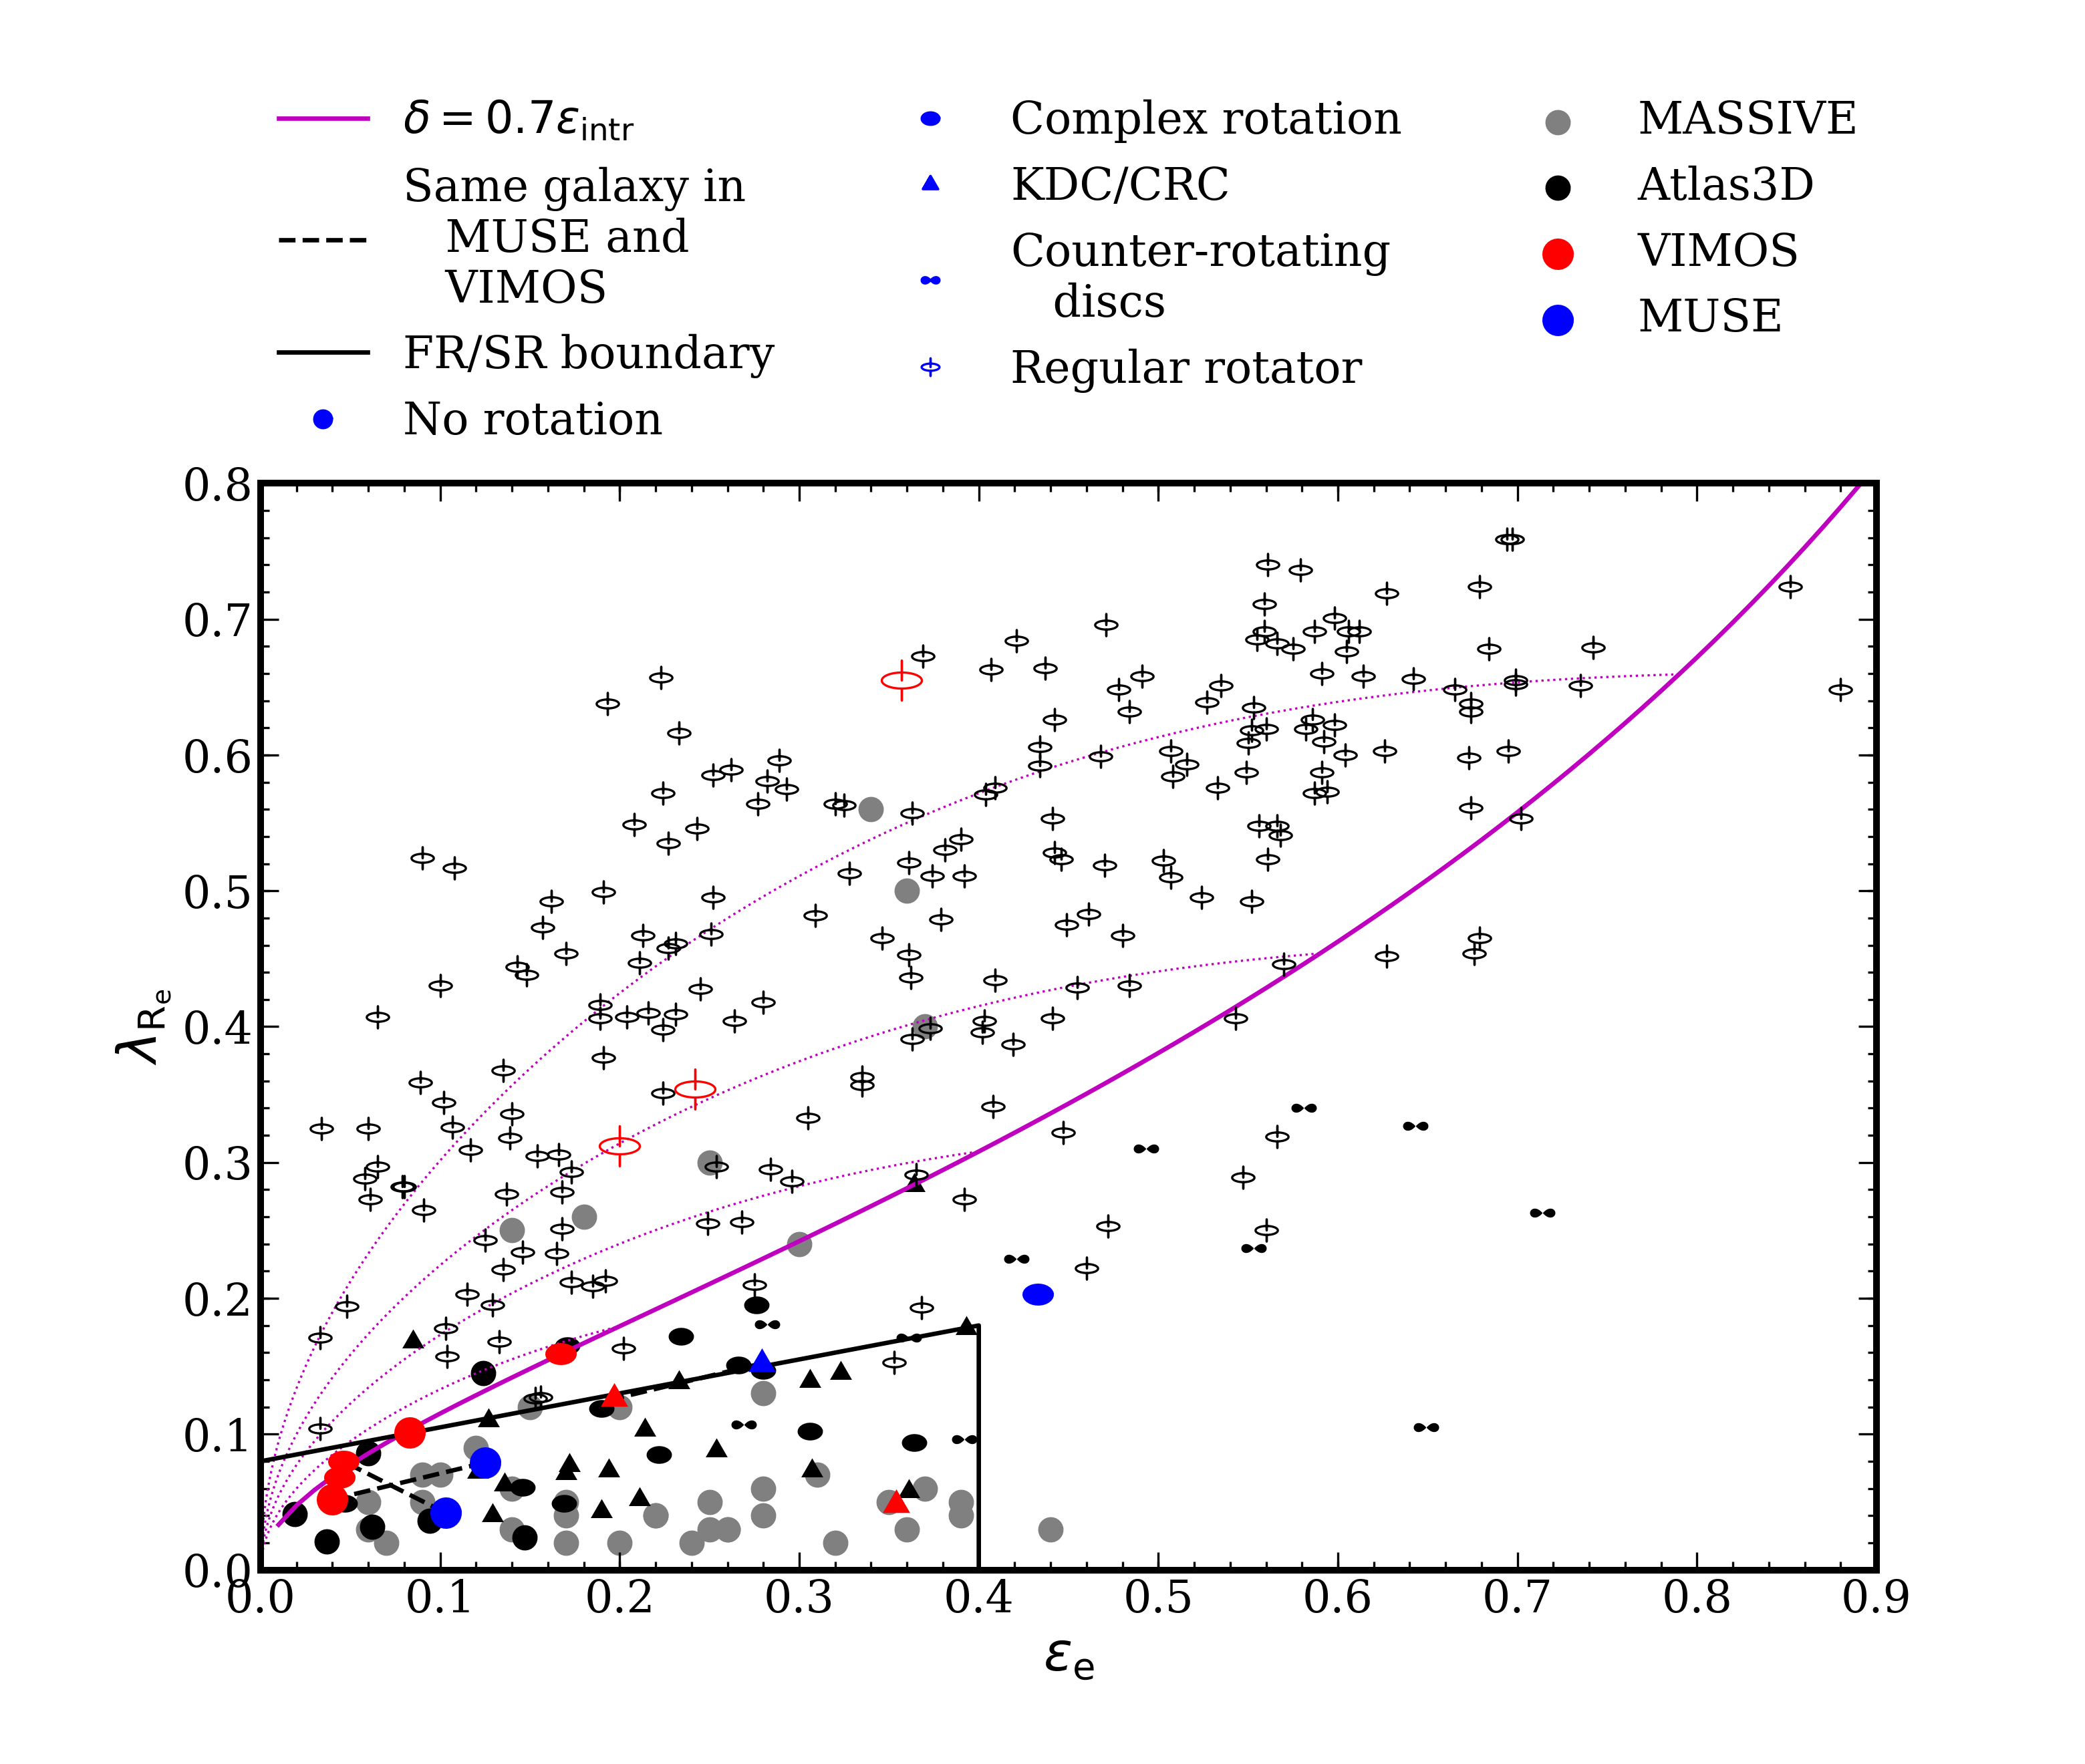
\includegraphics[width=\columnwidth]{lambda_R_ellipticity.png}
  \caption{$\lambda_\mathrm{R_e}$\,--\,ellipticity diagram. Our
    Southern Sample VIMOS and MUSE measurements are shown in red and
    blue, respectively. For comparison, Atlas$^\text{3D}$ galaxies
    \citep{Emsellem2011} are shown in black and MASSIVE galaxies
    \citep{Veale2017} in grey. Kinematic features are indicated by the
    symbol shape. The MASSIVE survey does not report substructure, so
    all MASSIVE sample galaxies are shown as filled circles. The
    theoretical limit (edge-on systems) of disc-dominated galaxies is
    indicated by the solid magenta line, with lines of constant
    intrinsic angular momentum but varying inclination in dotted
    magenta. The black solid lines indicate the limits of the
    fast-/slow-rotator classes. {\bf (In the figure legend, ``Regular
      Rotator'' should be ``Regular rotator''. The figure is also too
      small (the symbols can not be distinguished). Either put the
      legend on top or make the figure full width. Print it to check!
      Finally, for this and all figures except those of Appendix~B, it
      would be preferable to have small/minor tickmarks (with no
      numerical label) as well as large/major tickmarks.)}}
  \label{fig:lambdaR_ellip}
\end{figure}

\begin{figure}
  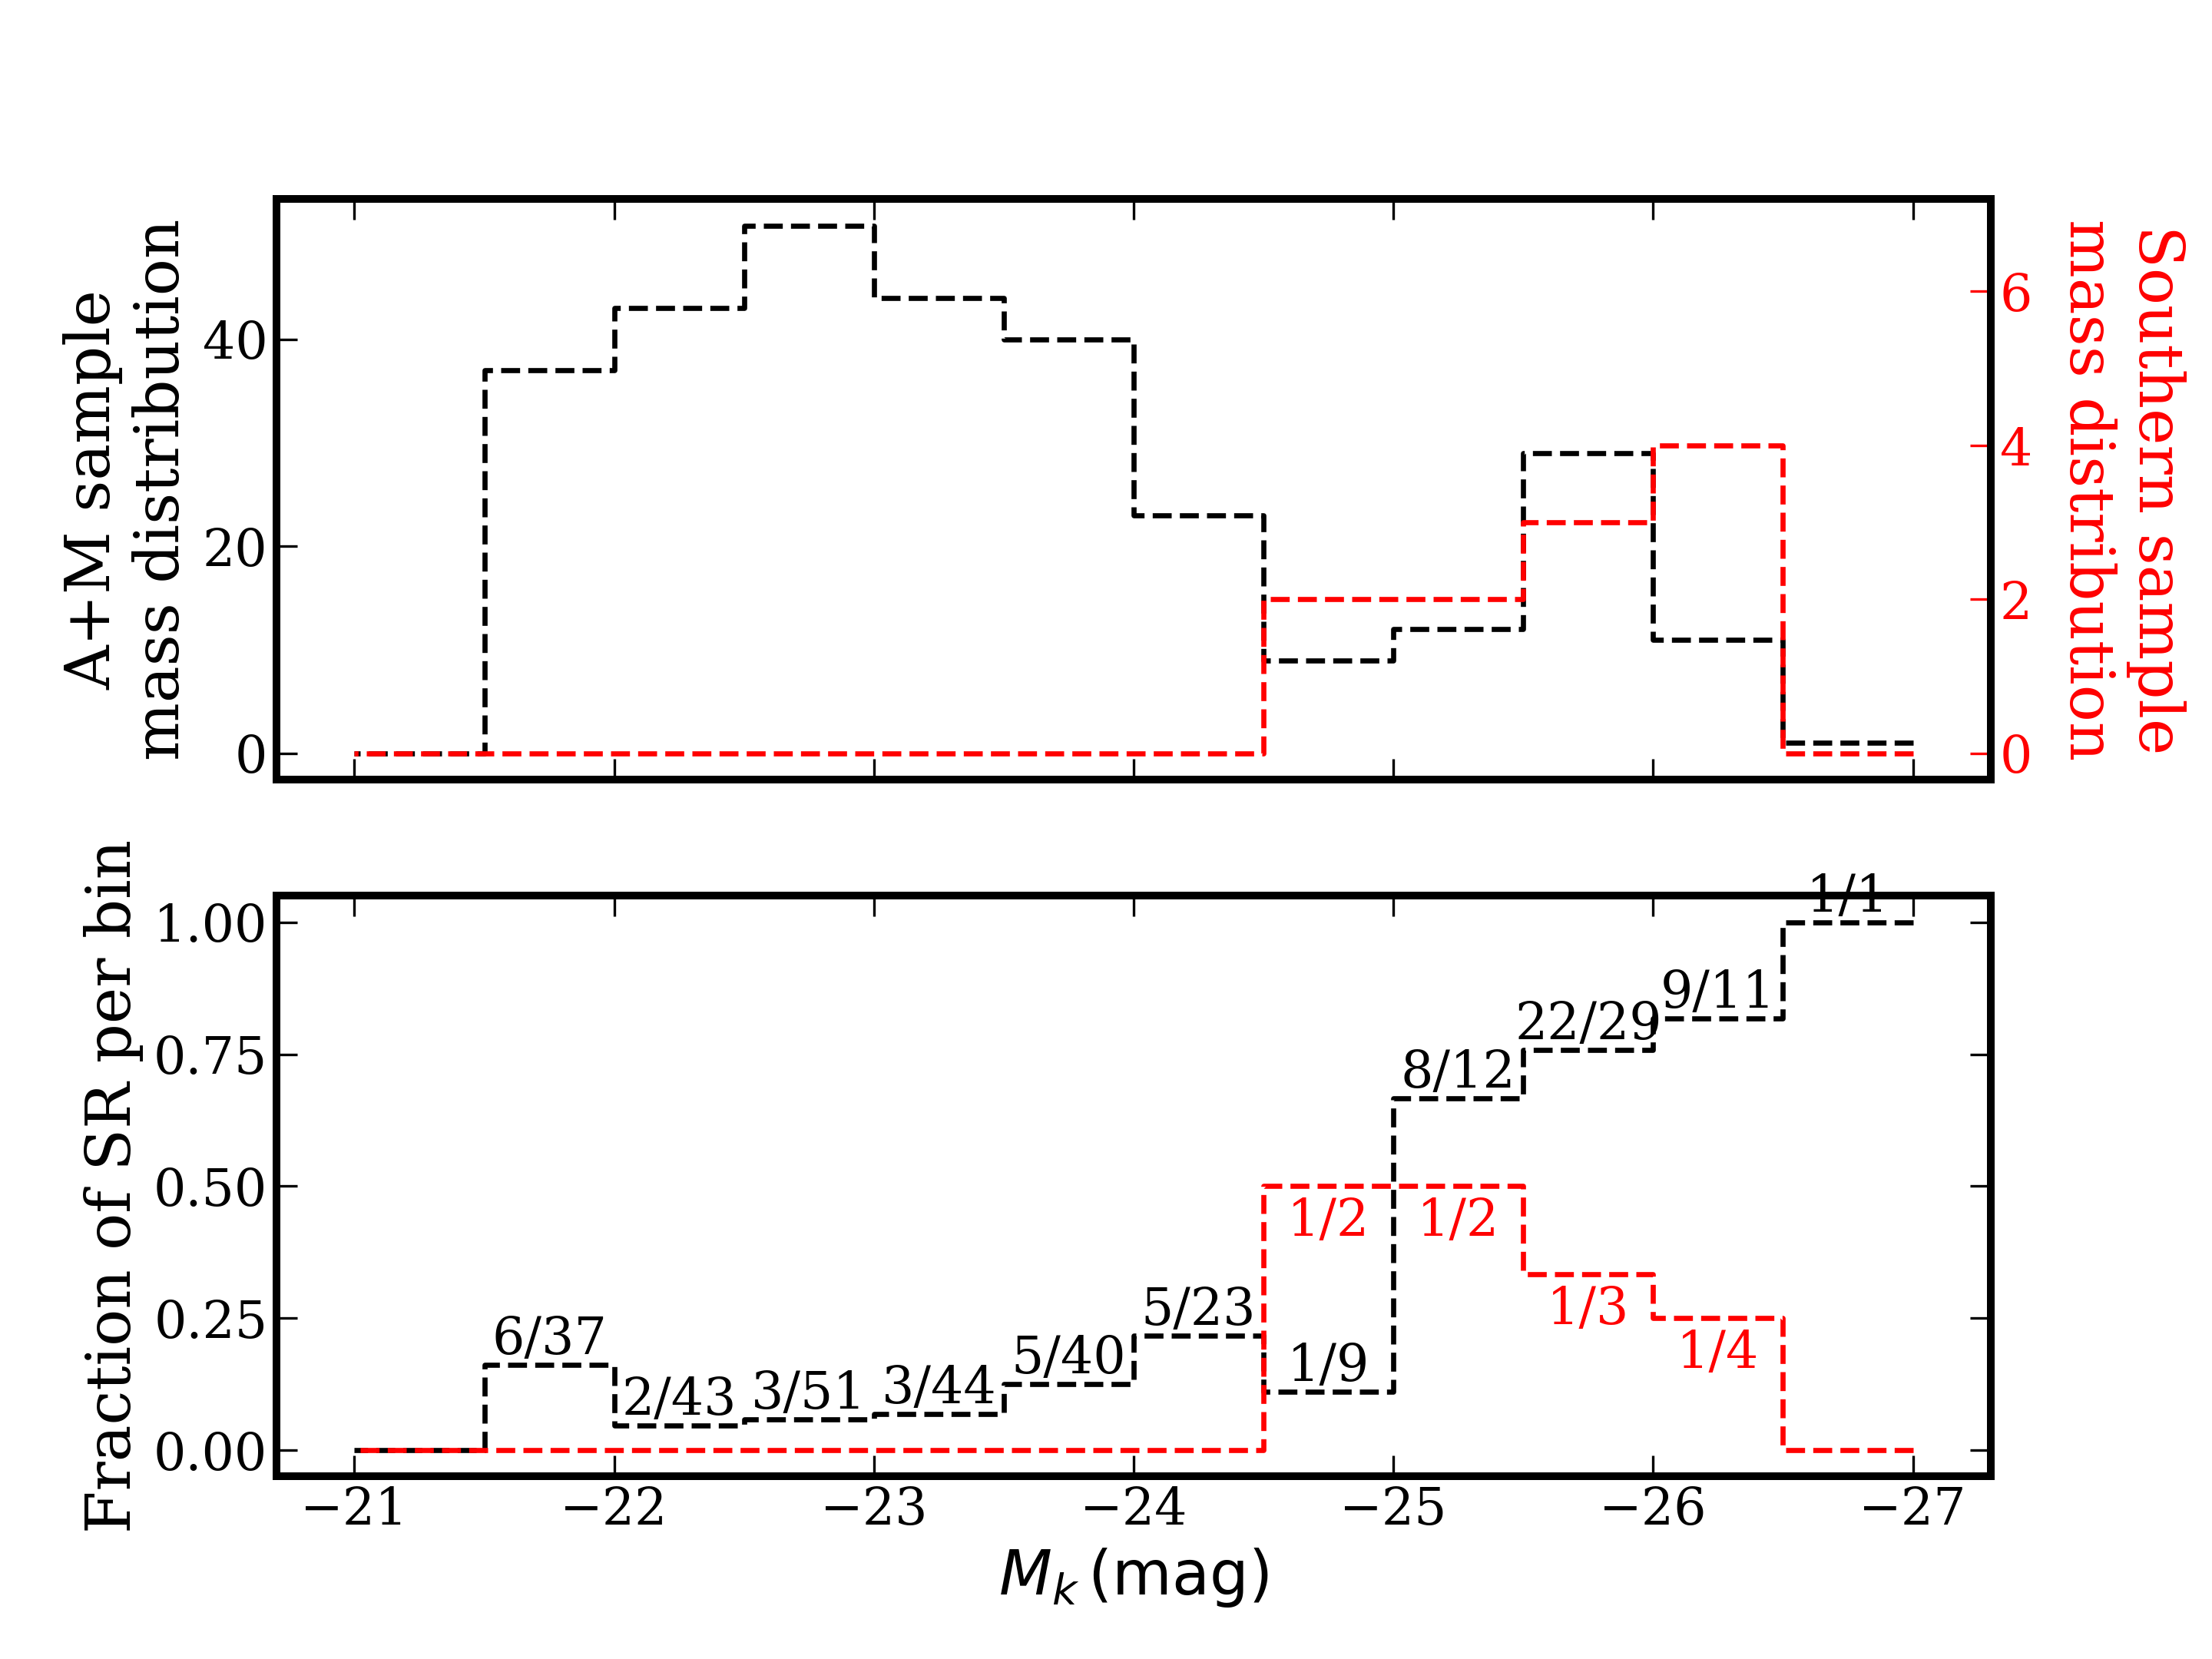
\includegraphics[width=\columnwidth]{M_k_binned.png}
  \caption{Upper panel: mass distribution of our Southern Sample (red,
    right axis) and the A+M sample (black, left axis). Lower panel:
    fraction of slow rotators within each mass bin, again
    colour-coded. The labels list the number of slow rotators and
    total number of galaxies in each bin. {\bf (In the y-axis label,
      ``Southern sample'' should be ``Southern Sample''.)}}
  \label{fig:SRmassFraction}
\end{figure}
                      
To account for the differences of the mass distributions, we find the
expected fraction of slow rotators in our Southern sample, $f'$,
corrected to the mass distribution of the A+M sample, as
\begin{equation}
  f^\prime=\frac{\sum_{i=0}^N\,N^\mathrm{SS}_if^\mathrm{AM}_i}{\sum_{i=0}^N\,N^\mathrm{SS}_i}~, 
\end{equation}
where $N^\text{SS}_i$ is the number of Southern Sample galaxies in the
$i^\text{th}$ mass bin, $f^\text{AM}_i$ is the fraction of slow
rotators in the $i^\text{th}$ mass bin of the A+M sample, and the sum
is computed over all $N$ mass bins. Here, we use the integrated
$K$-band absolute magnitude ($M_K$) as a proxy for stellar mass, with
bins of $0.5$~mag. This yields an expected fraction of slow rotators
for our Southern sample galaxies of $f^\prime=0.64\pm0.06$, consistent
with our measured fraction of $45\pm13\%$. The large uncertainty
reflects the low number statistics of our Southern Sample. Once
differences in the mass distributions are taken into account, there is
therefore no discernible difference in the fraction of galaxies that
are slow rotators between our radio-selected Southern Sample and the
optically-selected A+M sample.

{\bf (At the moment, the bottom panel of Fig.~\ref{fig:SRmassFraction}
  is never referenced nor discussed anywhere. It should, even
  briefly. Add some discussion of it.)}

\subsection{Kinematic Features}
\label{subsec:kin_features}

We attempted to identify the kinematic features defined by
\citet{Krajnovic2011} in an algorithmic manner, but the artefacts from
the different VIMOS quadrants confused ellipse-fitting
algorithms. Only the maps derived from MUSE data were therefore
classified in this automated way. The kinematic features in the VIMOS
maps were identified by eye. The resulting classifications are listed
in Column~7 of Table~\ref{tab:classify}, and the corresponding
kinematic group to which a galaxy belongs (also defined by
\citealt{Krajnovic2011}) is listed in Column~8. We identify $3$
kinematically-decoupled cores (KDCs; although PKS~718-34 is only a
tentative classification), such that $29\pm19\%$ of non-regular
rotators in our Southern Sample definitely (not including PKS~718-34)
contain a KDC (or $43\pm19\%$ including PKS~718-34), the large
uncertainty again reflecting the low-number statistics. This is
consistent with the Atlas$^\text{3D}$ survey, that found $25\pm7\%$ of
non-regular rotators hosting a KDC \citep{Krajnovic2011}.

\subsection{Intrinsic Shape}
\label{subsec:int_shape}

The misalignment angle $\Gamma_\text{kin}$ between the photometric and
kinematic position angles is listed in Column~4 of
Table~\ref{tab:classify}. IC~1531, NGC~7075 and PKS~718-34 all have
very large $PA_\text{phot}$ uncertainties, again due to the different
VIMOS quadrant artefacts causing the \textsc{kinemetry} fitting
routine to become unreliable.

{\bf (A solution to these large $PA_\text{phot}$ uncertainties would
  be to measure $PA_\text{phot}$ not from the surface brightness maps
  reconstructed from the IFS data, but rather from actual images, of
  which there should be many easily available. Of course, you would
  then need to make sure you know the orientation of these images
  accurately. Try it?)}

While intrinsically misaligned systems may appear aligned in certain
projections, aligned systems will be aligned in all
projections. Therefore, a low value of $\Gamma_\text{kin}$ cannot be
used to describe the intrinsic shape of an individual galaxy, but can
only be interpreted within a statistical framework (as in
\citealt{Cappellari2007}). However, a high value of
$\Gamma_\text{kin}$ does provide insight into the intrinsic shape of
an individual galaxy. Here, we find all the regular rotators in our
Southern Sample to be consistent with having aligned photometric and
kinematic position angles (to within $11\degr$), while non-regular
rotators have a large range of $\Gamma_\text{kin}$.

The lack of misalignments in regular rotators is consistent with
\citet{Cappellari2007}, \citet{Krajnovic2011} and \citet{Fogarty2015},
who all showed that regular rotators almost always have aligned
photometric and kinematic axes, with very little scatter. They also
pointed out that regular rotators with a significant misalignment tend
to be either interacting or strongly barred disc galaxies. This lack
of misalignments thus suggests that the regular rotators (including
those in our Southern Sample) are consistent with being axisymmetric
\citep{Cappellari2016}.

Misalignments between the photometric and kinematic position angles
are routinely observed for non-regular rotators. This generally
implies a more triaxial intrinsic shape, although large misalignments
are extremely rarely observed in galaxies with $\epsilon>0.4$,
suggesting that non-regular rotators are also more closely spherical
\citep{Cappellari2016}. The non-regular rotators in our Southern
Sample indeed all have $\epsilon<0.4$, with a broad range of
misalignment angles, and are thus consistent with fairly spherical
but mildly triaxial intrinsic shapes.

\section{Absorption Line Strengths}
\label{sec:absorption}

Using the methods described in Section~\ref{subsec:absorption}, we
produce maps of the absorption line strength indices for each galaxy
(shown in Appendix~\ref{sec:maps}). In this section, we thereafter
measure the relation between Mg and stellar velocity dispersion and
compare our absorption line strength measurements to other
measurements in the literature.

\subsection{Mg\,--\,$\sigma$ relation}
\label{subsec:Mg-sigma}

% The Mg$_2$ absorption line index of \citet{Trager1998} has
% overlapping bandpasses with the Mg\,b index (also of
% \citeauthor{Trager1998}), but includes the MgH molecular absorption
% line, and is hence considered a molecular index and is measured in
% units of magnitude.

\citet{Bender1993} observed a tight relationship between the \added{central} \removed{global}
Mg$_2$ absorption line strength (a variant of the Mg~$b$ line
strength) and the logarithm of the central stellar velocity
dispersion, $\sigma_0$, in elliptical galaxies. \removed{They also noticed that
the residuals from the best-fitting linear relation appeared to be
intrinsic, with a near Gaussian distribution about the median value}
{\bf (Was that median value $\approx0$? If so, state explicitly. If
  not, then the fit was either bad or there is something we do not
  understand.)} \removed{and no correlation with any other galaxy property.}

Part of the red continuum band of the Mg$_2$ index is outside the
spectral range of VIMOS, but \citet{Ziegler1997} showed there is an
approximately linear relationship between Mg~$b$ and Mg$_2$, with a
gradient of $14.3$\,--\,$15.5$~mag~\AA$^{-1}$ depending on
metallicity. {\bf (Why the strange units? Is Mg$_2$ measured in mag 
rather than \AA? If so, add a short note. If not, correct.)} 
\added{(Mg$_2$ is condered to be a molecular index and is thus measured 
in units of mag$^{-1}$.) We can thus}\removed{Thus, following \citet{Ziegler1997}, we also} use Mg~$b$ as a proxy for
Mg$_2$.

Using a central circular aperture with a radius of $2\arcsec$ in each
datacube, we measure $\sigma_0$ and Mg~$b$ at a degraded spectral
resolution of $8.4$~\AA\ full-width at half-maximum (FWHM), chosen
such that the transformation functions of \citet{Vazdekis2010} can be
used to change literature measurements from the Lick/IDS system to the
LIS. The results are shown in Fig.~\ref{fig:globalMg}, with the
best-fitting linear relationship
% (found using \textsc{lts\_linefit} from \citealt{Cappellari2013})
indicated by the solid black line, with a gradient of
$3.3\pm1.0$~\AA~dex$^{-1}$. \added{We} \removed{It was} noted that NGC~1316 is \added{again an} \removed{a possible}
outlier. {\bf (Noted by who or where? Specify. Also mention that it
  seems to again be an outlier here.)} Excluding NGC~1316 from the fit
yields a gradient of $2.5\pm0.7$~\AA~dex$^{-1}$ (green dashed line in
Fig.~\ref{fig:globalMg}). Both fits are in very good agreement with
the gradient found by \citet{Ziegler1997} for a sample of elliptical
galaxies in the Virgo and Coma clusters of galaxies
% using data from \citet{Dressler1987}
($2.7$~\AA~dex$^{-1}$, transformed to the LIS system using the
functions of \citealt{Vazdekis2010}; blue dotted line in
Fig.~\ref{fig:globalMg}). {\bf (Any uncertainty on this value of
  $2.7$? If so, quote it.) JW: No \citet{Ziegler1997} doesn't propagate uncertainty into errors on the fit.}
% , with an intrinsic scatter of 0.16\,\AA\ for galaxies with
% $\log \sigma_0 \geqslant 2.3$\,dex.

{\bf (One element I find confusing in this sub-section is that the
  first paragraph mentions a ``global'' relation, but the third
  paragraph and Fig.~3 use central $2\arcsec$ radius apertures that
  are therefore ``central'' apertures. Which one is right? You need to
  harmonise this. Also, in Fig.~\ref{fig:globalMg}, are you using the
  full relation of \citet{Ziegler1997} or just their gradient (and you
  then select a zero-point that suits you)? If the latter, then you
  must state this in the text. In other words, is the near perfect
  match of the green dashed and blue dotted lines truly a result or is
  it partially by construction (i.e.\ because you matched the
  zero-points yourself)? Clarify.) JW: the entire function has been transformed including the zero-point. This actually results in a cubic function (see Appendix A of \citealt{Vazdekis2010}), though as can been seen from the Fig.~3, the quadradic and cubic terms have very little effect in this range.}

\begin{figure}
  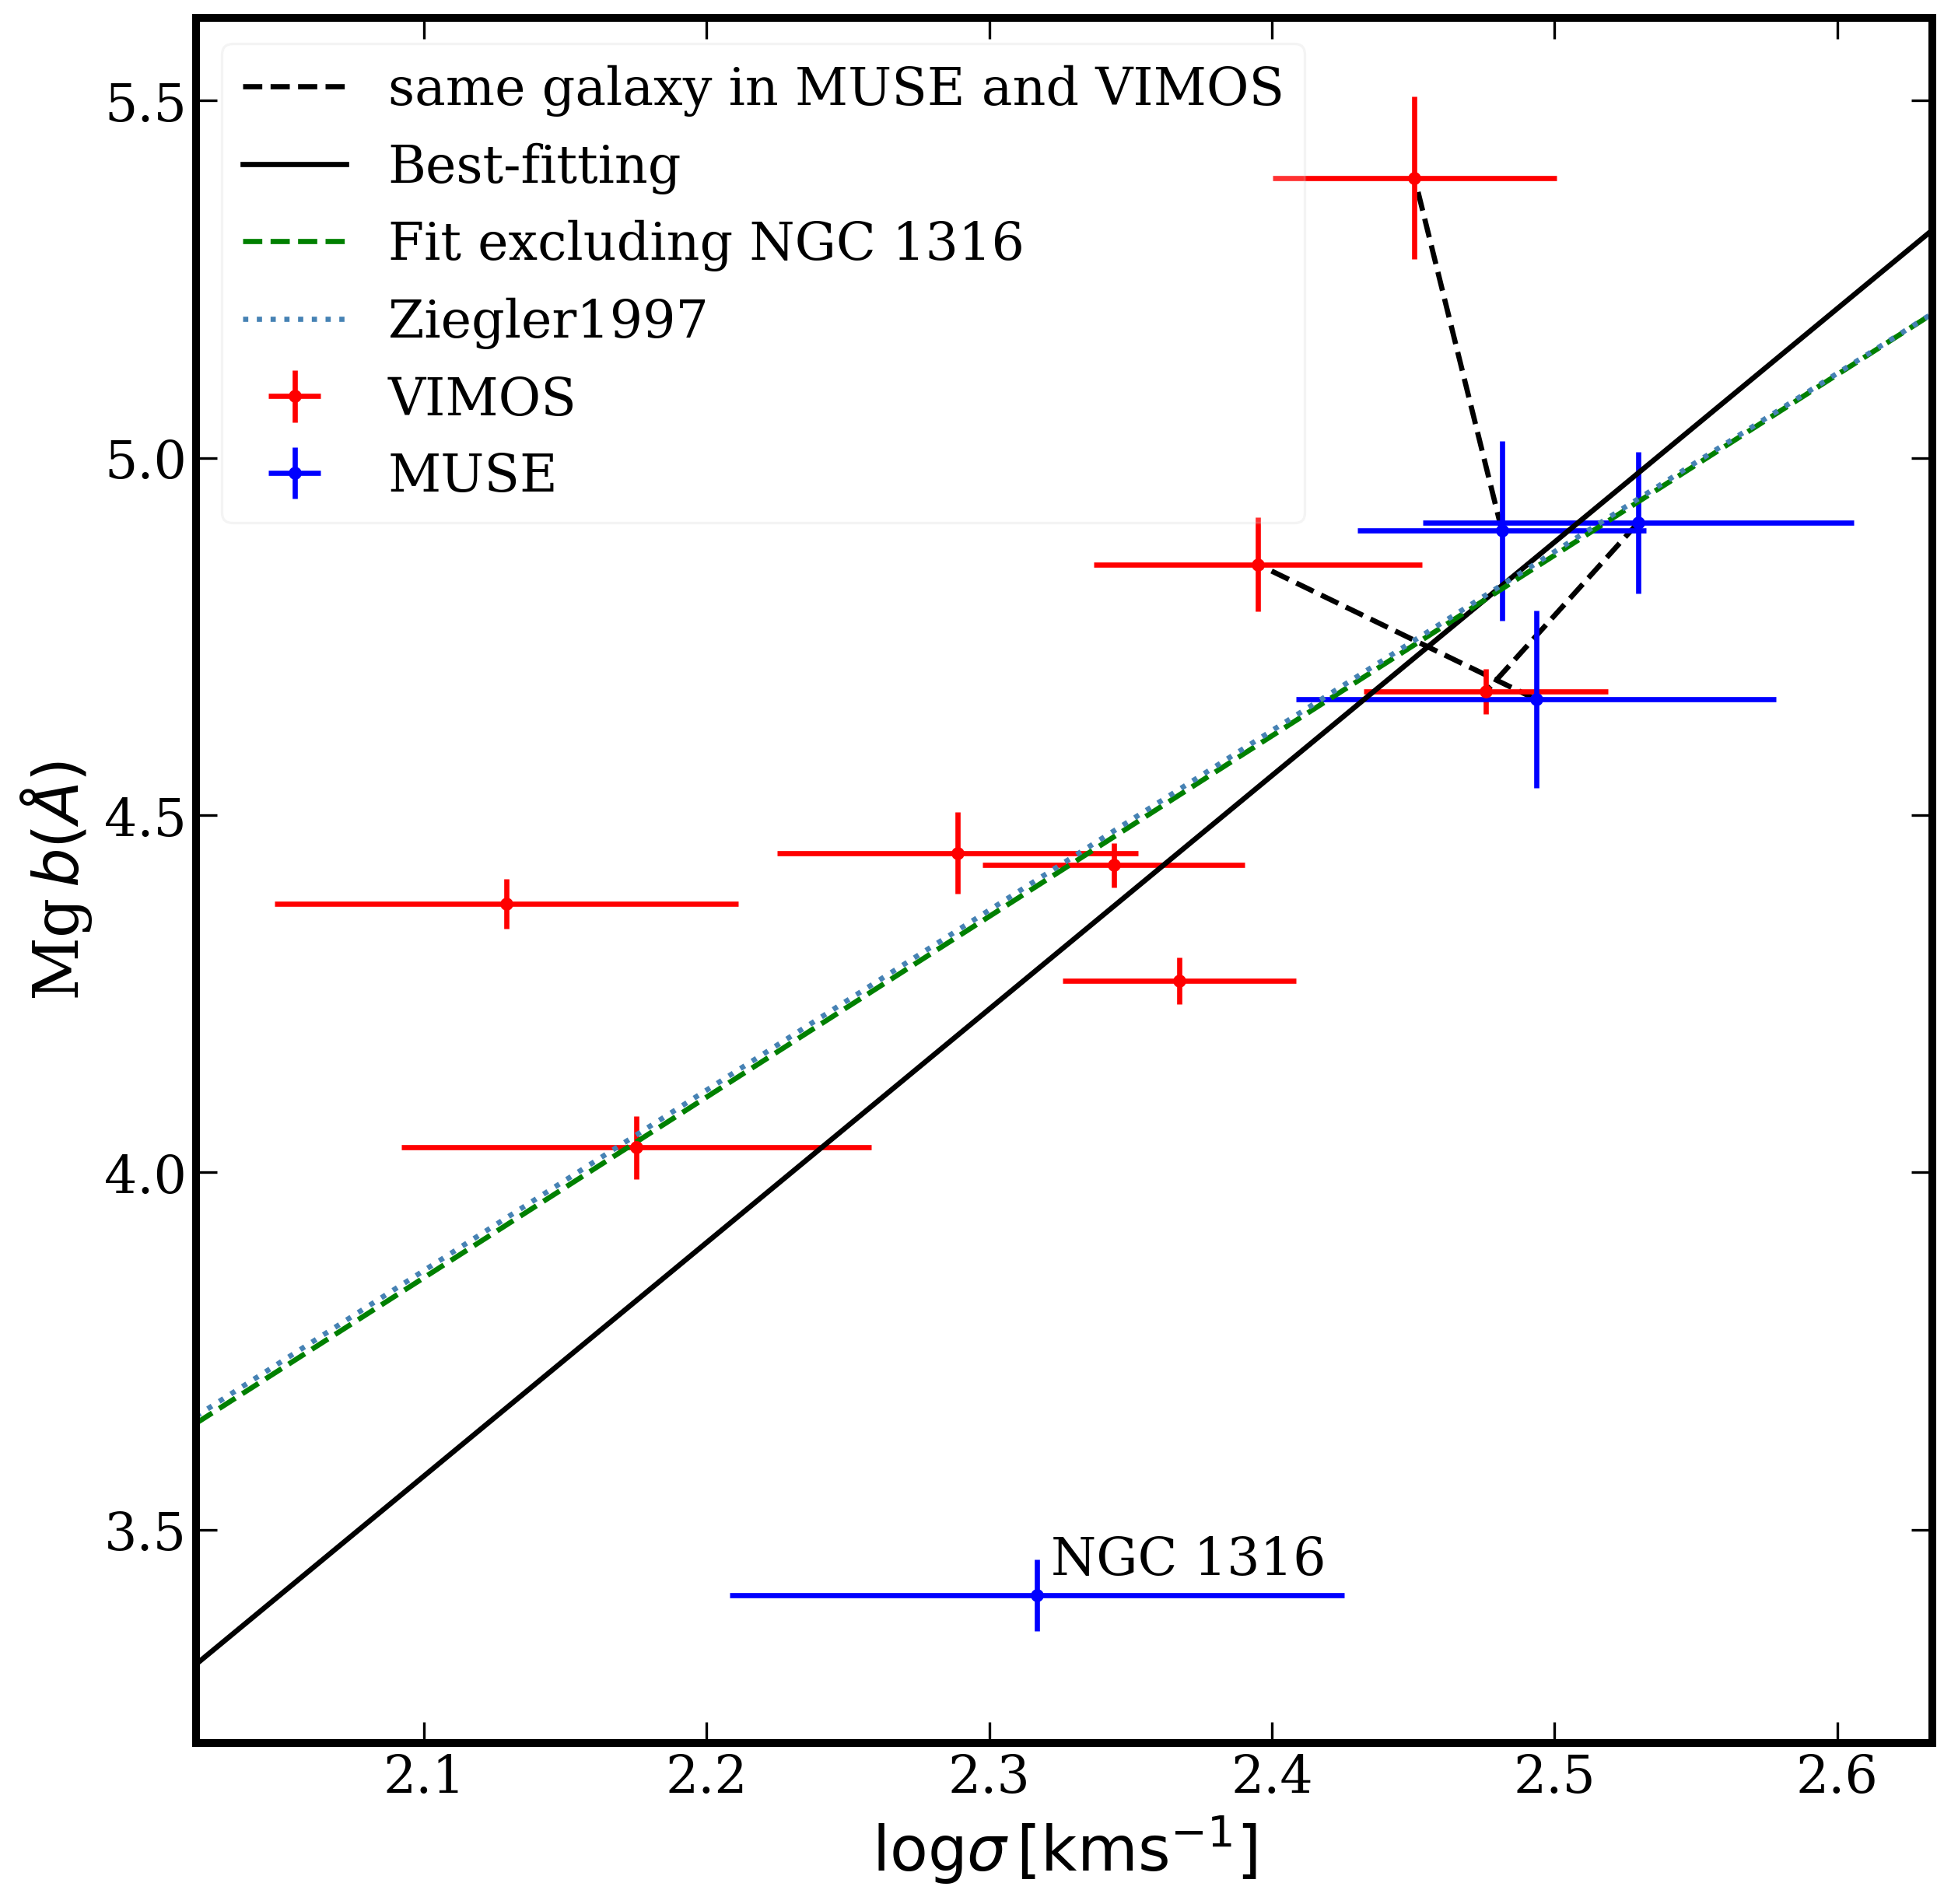
\includegraphics[width=\columnwidth]{Mg_sigma.png}
  \caption[Global Mg\,b\,--\,$\sigma$]{The Mg~$b$\,--\,central stellar
    velocity dispersion relation, using a central circular aperture of
    $2\arcsec$ radius. VIMOS and MUSE measurements are shown in red
    and blue, respectively. The best-fitting linear relation (solid
    black line) has a similar gradient to that found by
    \citeauthor{Ziegler1997} (\citeyear{Ziegler1997}; transformed to
    LIS using the functions of \citealt{Vazdekis2010}; blue dotted
    line). Removing NGC~1316 from the fit (green dashed line) results
    in a nearly perfect agreement (the green dashed and blue dotted
    lines are essentially indistinguishable). {\bf (In the legend,
      ``same'' should be ``Same'', ``Ziegler97'' should be ``Ziegler
      \& Bender (1997)'', and ``Fit excluding...'' should be
      ``Best-fitting excluding...''. In the y-axis label, there should
      be a space between ``$b$'' and ``(\AA)''. The x-axis label
      should be ``$\log\,(\sigma_0/{\rm km~s^{-1}})$''.)}}
  \label{fig:globalMg}
\end{figure}

\subsection{Comparisons to the Literature}
\label{subsec:Lit}

Given that there is no well-defined list of corrections (or correction
methods) that is universally accepted, care must be taken when
comparing different line strength measurements. In what follows, when
comparing to the measurements reported in a specific paper, we
therefore correct for the same effects described in that paper, but
using our methods (see Section~\ref{subsec:absorption}). To provide a
fair comparison between indices, and to have the benefit of the
transformation functions of \citet{Vazdekis2010} for literature
measurements, we again use a degraded spectral resolution of
$8.4$~\AA\ FWHM (see Section~\ref{subsec:Mg-sigma}).

Table \ref{tab:litAbsorption} summarises our comparisons to multiple
sets of literature measurements, where the offsets and dispersions
listed are defined as the means and standard deviations of the
differences between the literature measurements and ours. For the
comparison to \citet{Vazdekis2010}, we re-analysed the Spectral Aeral
Unit for Research on Optical Nebulae (SAURON)
dataset\footnote{\url{http://www.strw.leidenuniv.nl/sauron/}}
\citep{Emsellem2004} using the same analysis pipeline as for our
Southern Sample. {\bf (Why not use the much larger Atlas$^{\rm 3D}$
  dataset instead? Explain briefly if justified.)} \added{This was used over the larger Atlas$^\text{3D}$ sample \citep{Cappellari2011}, as stellar populations were not published by the Atlas$^\text{3D}$ team.}

\begin{table}
  \begin{center}
  % \begin{threeparttable}
    \caption{Comparisons of measured and literature absorption line
      strength measurements.}
    \label{tab:litAbsorption}
    \begin{tabular*}{0.4\textwidth}{@{\extracolsep{\fill}}l r r r}
      \hline
      \hline
      Index 		& \multicolumn{1}{c}{$N_\mathrm{gals}$} & \multicolumn{1}{c}{Offset} & \multicolumn{1}{c}{Dispersion} \\
                        & 		& \multicolumn{1}{c}{(\AA)} & \multicolumn{1}{c}{(\AA)} \\
      \hline
      \multicolumn{4}{c}{\citet{Vazdekis2010} (SAURON)} \\
      \hline
      H$\beta$  	& $46$		& $-0.02\leavevmode\phantom{0}$ & $0.25\leavevmode\phantom{0}$\\
      Fe5015		& $46$		& $0.66\leavevmode\phantom{0}$ & $0.34\leavevmode\phantom{0}$\\
      Mg~$b$ 		& $46$		& $0.06\leavevmode\phantom{0}$ & $0.33\leavevmode\phantom{0}$\\
      \hline
      \multicolumn{4}{c}{\citet{Rampazzo2005} (VIMOS)} \\
      \hline
      G4300 		& $3$ 		& $2.29\leavevmode\phantom{0}$ & $0.11\leavevmode\phantom{0}$\\
      Fe4383 		& $3$ 		& $0.39\leavevmode\phantom{0}$ & $0.23\leavevmode\phantom{0}$\\
      Ca4455 		& $3$ 		& $-0.19\leavevmode\phantom{0}$ & $0.09\leavevmode\phantom{0}$\\
      Fe4531 		& $3$ 		& $0.16\leavevmode\phantom{0}$ & $0.26\leavevmode\phantom{0}$\\
      H$\beta$  	& $3$ 		& $0.17\leavevmode\phantom{0}$ & $0.12\leavevmode\phantom{0}$\\
      Fe5015 		& $3$ 		& $-0.73\leavevmode\phantom{0}$ & $0.48\leavevmode\phantom{0}$\\
      Mg~$b$		& $3$ 		& $-0.43\leavevmode\phantom{0}$ & $0.17\leavevmode\phantom{0}$\\
      \hline
      \multicolumn{4}{c}{\citet{Rampazzo2005} (MUSE)} \\
      \hline
      H$\beta$  	& $2$ 		& $-0.28\leavevmode\phantom{0}$ & $0.17\leavevmode\phantom{0}$\\ 
      Fe5015 		& $2$ 		& $0.87\leavevmode\phantom{0}$ & $0.34\leavevmode\phantom{0}$\\ 
      Mg~$b$ 		& $2$ 		& $0.31\leavevmode\phantom{0}$ & $0.14\leavevmode\phantom{0}$\\
      Fe5270 		& $2$ 		& $-0.11\leavevmode\phantom{0}$ & $0.15\leavevmode\phantom{0}$\\
      Fe5335 		& $2$ 		& $0.08\leavevmode\phantom{0}$ & $0.15\leavevmode\phantom{0}$\\
      Fe5406 		& $2$ 		& $0.16\leavevmode\phantom{0}$ & $0.07\leavevmode\phantom{0}$\\
      Fe5709 		& $2$ 		& $0.11\leavevmode\phantom{0}$ & $0.10\leavevmode\phantom{0}$\\
      Fe5782 		& $2$ 		& $-0.03\leavevmode\phantom{0}$ & $0.11\leavevmode\phantom{0}$\\
      NaD 		& $2$ 		& $0.90\leavevmode\phantom{0}$ & $0.41\leavevmode\phantom{0}$\\
      TiO1 (mag)	& $2$ 		& $-0.004$	& $0.003$\\
      TiO2 (mag)	& $2$ 		& $-0.011$	& $0.007$\\
      \hline
      \multicolumn{4}{c}{\citet{Ogando2008} (VIMOS)} \\
      \hline
      H$\beta$  	& $6$ 		& $0.07\leavevmode\phantom{0}$ & $0.60\leavevmode\phantom{0}$\\
      Fe5015 		& $6$ 		& $-0.09\leavevmode\phantom{0}$ & $0.15\leavevmode\phantom{0}$\\
      Mg~$b$ 		& $6$ 		& $-0.70\leavevmode\phantom{0}$ & $0.08\leavevmode\phantom{0}$\\
      \hline
      \multicolumn{4}{c}{\citet{Ogando2008} (MUSE)} \\
      \hline
      H$\beta$  	& $3$ 		& $-0.04\leavevmode\phantom{0}$ & $0.23\leavevmode\phantom{0}$\\ 
      Fe5015 		& $3$ 		& $-0.16\leavevmode\phantom{0}$ & $0.33\leavevmode\phantom{0}$\\ 
      Mg~$b$ 		& $3$ 		& $-1.10\leavevmode\phantom{0}$ & $0.26\leavevmode\phantom{0}$\\
      Fe5270 		& $3$ 		& $-0.66\leavevmode\phantom{0}$ & $0.16\leavevmode\phantom{0}$\\
      Fe5335 		& $3$ 		& $-0.66\leavevmode\phantom{0}$ & $0.11\leavevmode\phantom{0}$\\
      Fe5406 		& $3$ 		& $-0.51\leavevmode\phantom{0}$ & $0.06\leavevmode\phantom{0}$\\
      Fe5709 		& $3$ 		& $-0.22\leavevmode\phantom{0}$ & $0.08\leavevmode\phantom{0}$\\
      NaD 		& $3$ 		& $-1.57\leavevmode\phantom{0}$ & $0.16\leavevmode\phantom{0}$\\
      \hline
      \hline
    \end{tabular*}
    % \begin{tablenotes}
    \parbox[t]{0.4\textwidth}{\footnotesize\textit{Notes:} Comparisons
      to \citet{Rampazzo2005} are sampled at $7$ radial apertures for
      each galaxy: $1.5$, $2.5$ and $10\farcs0$, and $R_\text{e}/10$,
      $R_\text{e}/8$, $R_\text{e}/4$ and $R_\text{e}/2$. Col.~1: Line
      strength index. Col.~2: Number of galaxies in
      comparison. Cols.~3 and 4: Mean and standard deviation of the
      differences between the literature measurements and ours.}
  \end{center}
  % \end{tablenotes}
  % \end{threeparttable}
\end{table}

We find a very large offset between the G4300 index measurements of
\citet{Rampazzo2005} and ours. This index is however extremely
sensitive to the stellar velocity dispersion correction, and we
measure an average difference of the stellar velocity dispersions
measured by \citet{Rampazzo2005} and us of $21$~km~s$^{-1}$. 
\removed{This may be enough to account for the offset of the measurements.} {\bf (Why not
  check this by changing the stellar velocity dispersions used in your
  corrections to those of \citealt{Rampazzo2005}? Check. JW: I can't get anywhere close the values of Rampazzo for G4300. Once the conversion to LIS is included, I have to double the stellar velocity dispersion, before I get can get similar results! I'm not sure what to do about this.)}

\removed{The offsets of our Fe5015 index measurements are also relatively large
when compared to the measurements of \citet{Rampazzo2005} and
\citet{Vazdekis2010}. The origin of this offset is unclear for the
latter, but for the former it may be due to differences in the way the
[\ion{O}{iii}] doublet emission is accounted for.} {\bf (In both cases,
  the offsets are smaller than $3\sigma$, in the sense that the stated
  offset is less than $3$ times the stated dispersion. The offsets are
  thus not really significant... is this discussion therefore really
  worth it? A number of other indices from \citealt{Rampazzo2005} also
  show equally significant offsets ($\approx2\sigma$). What about
  them? I think this notion of the ``significance'' of the offsets
  must be introduced/addressed to justify which offsets you choose to
  discuss.)}

\removed{Indices other than G4300 and Fe5015 generally have literature
measurements that are fairly consistent with ours, although the
dispersions of the measurements are fairly large (perhaps due to the
transformations from Lick to LIS system indices).}
{\bf (A number of the offsets listed in the table actually {\em are}
  significant (i.e.\ $>3\sigma$). In particular, a majority of the
  offsets with the \citealt{Ogando2008} measurements are
  significant. Why are these measurements so inconsistent? I think
  this should be discussed.)}

\added{For many indices \citet{Ogando2008} found significantly stronger measurements to us.} {\bf JW: I need help with this part, I don't know how to explain why they might be different - all I can say is that are.}

\section{Stellar Populations}
\label{sec:stellarPop}

{\bf (Here, you just straightaway jump into a discussion of the
  stellar populations, i.e.\ the derived quantities of age and
  metallicity. I think this should be preceded (possibly in the
  previous section) by a discussion of the line strengths themselves,
  at least in the same spirit as what is done here for the
  populations, i.e.\ radial gradients and KDCs (that are not discussed
  in the preceding section on line strengths, that exclusively deals
  with Mg\,--\,$\sigma$ and the litetature comparison). Add?)}

Assuming that the individual spectra from our Southern Sample galaxies
can be well approximated by a SSP, we use the methods and the
absorption line strength maps described in
Section~\ref{subsec:absorption} to produce maps of the most-likely \added{luminosity-weighted} SSP
parameters (see Appendix~\ref{sec:maps}): age ($t$), metallicity
\removed{($Z/H$)}\added{($[M/H]$)} and alpha-element enhancement ($\alpha$/Fe). {\bf (You must
  specify here (and presumably also in
  Section~\ref{subsubsec:stellarPop}) whether the stellar population
  parameters are mass- or luminosity-weighted.)}

{\bf (I am confused here because in the paragraph above you refer to
  $Z/H$ as your proxy for metallicity, but in the paragraph below you
  keep talking about [Fe/H], and in the maps the labels are just
  ``metalicity'' (yes, with the spelling mistake!). Which one is right
  (metallicity, $Z/H$, [$Z/H$], Fe/H or [Fe/H]? Use only the right one
  and be consistent.)}

In general, our Southern Sample galaxies show old, metal-rich and
alpha-enhanced SSPs, characteristics that are common in ETGs \added{\citep[e.g.][]{Worthey1992}}{\bf (Add
  a classic reference here.)} The exceptions are NGC~612 and
NGC~1316. NGC~1316 has a very young stellar population (our fit of
$t\approx2$~Gyr is consistent with that of \citealt{Kuntschner2000},
but is conflicting with the older and less metal-rich estimate of
\citealt{Koleva2011}, who found $t=4.5\pm0.3$~Gyr and
\removed{$\mathrm{[Fe/H]}=0.12\pm0.01$}\added{$\mathrm{[M/H]}=0.12\pm0.01$} \removed{for an aperture covering the central
$0.1$~kpc)}`added{using a long slit with width $1\arcsec$ and length $0.1$~kpc)}. {\bf (Is that a circular or square aperture? If circular,
  is $0.1$~kpc the radius or diameter? Clarify.)} We also find NGC~612
to have an extended young stellar population of
$t\approx4$~Gyr. Otherwise, NGC~3557 is notable for containing a
significantly younger ($t\approx4$~Gyr) core of $\approx10\arcsec$ in
diameter, and NGC~3100 has a branch of young stars ($t\approx4$\,Gyr) \added{with very high metallicity projecting southwards from below the eastern}
\removed{along the south-east} branch of the molecular gas (\removed{white} 
\added{cyan} contours in
Fig.~\ref{fig:ngc3100}). {\bf (I do not see the age feature you refer
  to in the NGC3100 maps, and the CO is distributed North-East to
  South-West, so there is no South-East CO ``branch''. Perhaps you
  meant South-West (where there is indeed a blue region in the
  H$\beta$ map, if not in the age map)? Also, there is no white
  contour in the figure. The CO contours are in pale
  blue/turquoise. Is that what you meant? In any case, this needs to
  be corrected to reflect the truth.)}

\subsection{Radial Gradients in Stellar Populations}
\label{subsec:popGrad}

\citet{Koleva2011} showed that while there are wide ranges of radial
gradients of age and metallicity across galaxy populations, the mean
gradients are approximately constant across a large mass range. To
probe this they assumed a linear relationship between $\log(t)$ or
\removed{[Fe/H]}\added{[M/H]} and $\log(R/R_\text{e})$, i.e.\ as is common the gradients
considered are logarithmic radial gradients. We repeated these fits
with our Southern Sample galaxies, and the results are listed in
Table~\ref{tab:derivedProp}.

\begin{table*}
  \begin{center}
    \caption{Derived stellar population and ionised gas properties of
      our Southern Sample galaxies.}
    \label{tab:derivedProp}
    \begin{tabular*}{0.95\textwidth}{@{\extracolsep{\fill}}l c c c c c c c c}
      \hline
      \hline 
      Galaxy & \multicolumn{2}{c}{$\Delta\log(t)$} & \multicolumn{2}{c}{\removed{$\Delta\text{[Fe/H]}$}\added{$\Delta\text{[M/H]}$}} & \multicolumn{2}{c}{$\log(M_\text{\ion{H}{ii}}/\mathrm{M_\odot})$} & Balmer Dec. & Ionisation\\
             & VIMOS & MUSE & VIMOS & MUSE & VIMOS$^\text{a}$ & MUSE & & \\
      \hline
      ESO~443-G024 & $0.019\pm0.013$ & -- & $-0.01\pm0.02$ & -- & $5.02\pm0.01$ & -- & -- & LINER \\
      IC~1459 & $0.005\pm0.015$ & $0.003\pm0.002$ & $-0.02\pm0.02$ & $0.00\pm0.06$ & $5.21\pm0.01$ & $5.50\pm0.01$ & $4.54\pm0.12$ & LINER-AGN \\
      IC~1531 & $0.012\pm0.015$ & -- & $\leavevmode\phantom{-}0.01\pm0.02$ & -- & $5.09\pm0.01$ & -- & -- & Seyfert 2\\
      IC~4296 & $0.012\pm0.010$ & $0.000\pm0.002$ & $-0.03\pm0.01$ & $0.04\pm0.08$ & $5.43\pm0.01$ & $< 4.48$ & $^\text{b}$ & LINER-AGN \\
      NGC~612 & $0.068\pm0.060$ & -- & $-0.11\pm0.02$ & -- & $6.00\pm0.01$ & --	& -- & LINER-AGN \\
      NGC~1316 & -- & $0.001\pm0.002$ & -- &$0.05\pm0.03$ & -- & $ 5.29\pm0.01$ & $3.52\pm0.11$ & LINER-AGN \\
      NGC~1399 & $0.019\pm0.005$ & $0.001\pm0.002$ & $-0.02\pm0.03$ & $0.10\pm0.09$ & $< 3.86$ & $ 4.54\pm0.01$ & $< 21.4^\text{c}$ & LINER \\
      NGC~3100 & $0.000\pm0.010$ & -- & $-0.06\pm0.01$ & -- & $5.26\pm0.01$ & -- & -- & LINER-AGN \\
      NGC~3557 & $0.048\pm0.039$ & -- & $-0.05\pm0.05$ & -- & $4.61\pm0.02$ & -- & -- & LINER \\
      NGC~7075 & $0.007\pm0.011$ & -- & $-0.07\pm0.02$ & -- & $4.68\pm0.01$ & -- & -- & LINER \\
      PKS~718-34 & $0.002\pm0.009$ & -- & $-0.17\pm0.03$ & -- & $< 5.08$ & -- & -- & Passive \\
      \hline
      \hline
    \end{tabular*}
    \parbox[t]{0.95\textwidth}{\footnotesize\textit{Notes:} Col.~1:
      galaxy name. Cols.~2\,--\,3: logarithmic radial age gradient of
      the most-likely SSP model. Cols.~4\,--\,5: logarithmic radial
      metallicity gradient of the most-likely SSP
      model. Cols.~6\,--\,7: \ion{H}{ii} mass derived from the
      H$\beta$ (assuming a Balmer decrement of $2.85$) or H$\alpha$
      line for the VIMOS or MUSE data, respectively. Col.~8: Balmer
      decrement measured from the MUSE data. Col.~9: Primary
      ionisation mechanism (see Section~\ref{subsec:Diagnostics} for a
      description of the different mechanisms).\\
      $^\text{a}$ The VIMOS flux calibration and thus the derived
      \ion{H}{ii} masses are only approximate (see
      Section~\ref{sec:obs} for more detail on the flux
      calibration).\\
      $^\text{b}$ Neither H$\alpha$ nor H$\beta$ is detected with
      $A/N>2.5$, so no useful Balmer decrement can be measured.\\
      $^\text{c}$ H$\beta$ is not detected with $A/N>2.5$, so the fit
      is unreliable and only an upper limit on the Balmer decrement
      (assuming an H$\beta$ detection with $A/N=2.5$) is reported.}
  \end{center}
\end{table*}
  
We find average logarithmic radial gradients of
$\Delta\log(t)=0.014\pm0.007$ and
\removed{$\Delta\text{[Fe/H]}=-0.03\pm0.01$}\added{$\Delta\text{[M/H]}=-0.03\pm0.01$}. These are consistent with the
results of \citet{Koleva2011}, who found average gradients of
respectively $0.06\pm0.09$ and $-0.26\pm0.08$ for elliptical galaxies,
and respectively $0.01\pm0.11$ and $-0.12\pm0.13$ (i.e.\ flatter) for
lenticular galaxies.

\subsection{Kinematically-decoupled Cores}
\label{subsec:popKDC}

\added{\citet{McDermid2006}} \removed{\citet{Kuntschner2010}} showed that 
KDCs can be separated into two classes: either small with various stellar 
ages or typically larger but containing a homogeneously old stellar 
population. {\bf (I thought the first to point this out was 
McDermid et al.\ (2006; see e.g.\ their Fig.~16), which should at 
least also be quoted here. Check and possibly correct.)} 
\added{Using the method of \citet{McDermid2006},} the size 
\added{and age} of the KDC is defined as the radius
where the superposition of the two kinematic components (the KDC and
the host galaxy) results in a local minimum in the mean velocity \added{and} the
age of the most-likely SSP model for the spatially integrated spectrum
within a central \added{, circular} aperture with a \added{radius} of 
$1\arcsec$ {\bf (Again, square or circular, radius or diameter? Clarify.)} 
\removed{is taken as the KDC's age.} \added{, respectively.} 
{\bf (Are these two definitions (of the KDCs' sizes and ages) 
those of \citealt{Kuntschner2010} or yours or both? Clarify.)}

The typical size of the smaller class of KDCs (always hosted by fast
rotators) is too small to be spatially resolved by our data, so these
KDCs are not considered here. The generally larger, old KDCs are
typically hosted by slow rotators \citep{Kuntschner2010}. They have no
upper limit on their stellar ages, i.e.\ they do not fade into their
host galaxies as they age unlike the small KDCs, suggesting the stars
within these large KDCs dominate in mass as well as surface
brightness. \citet{Bois2011} showed major mergers may well result in
such large KDCs if the initial spin axis of the progenitor galaxy with
the lowest bulge-to-disc ratio (i.e.\ the later-type galaxy) is
anti-parallel to its orbital angular momentum vector.

In Fig.~\ref{fig:KDC}, we show the age and size of each of the $3$
KDCs identified in our Southern Sample galaxies. We include the
PKS~718-34 KDC here, but we stress it is only tentatively classified
as a KDC. As can be seen from Fig.~\ref{fig:KDC}, the KDC of
PKS~718-34 would be extremely large, but nevertheless all $3$ KDCs are
consistent with those found by \citet{Kuntschner2010}.

\begin{figure}
  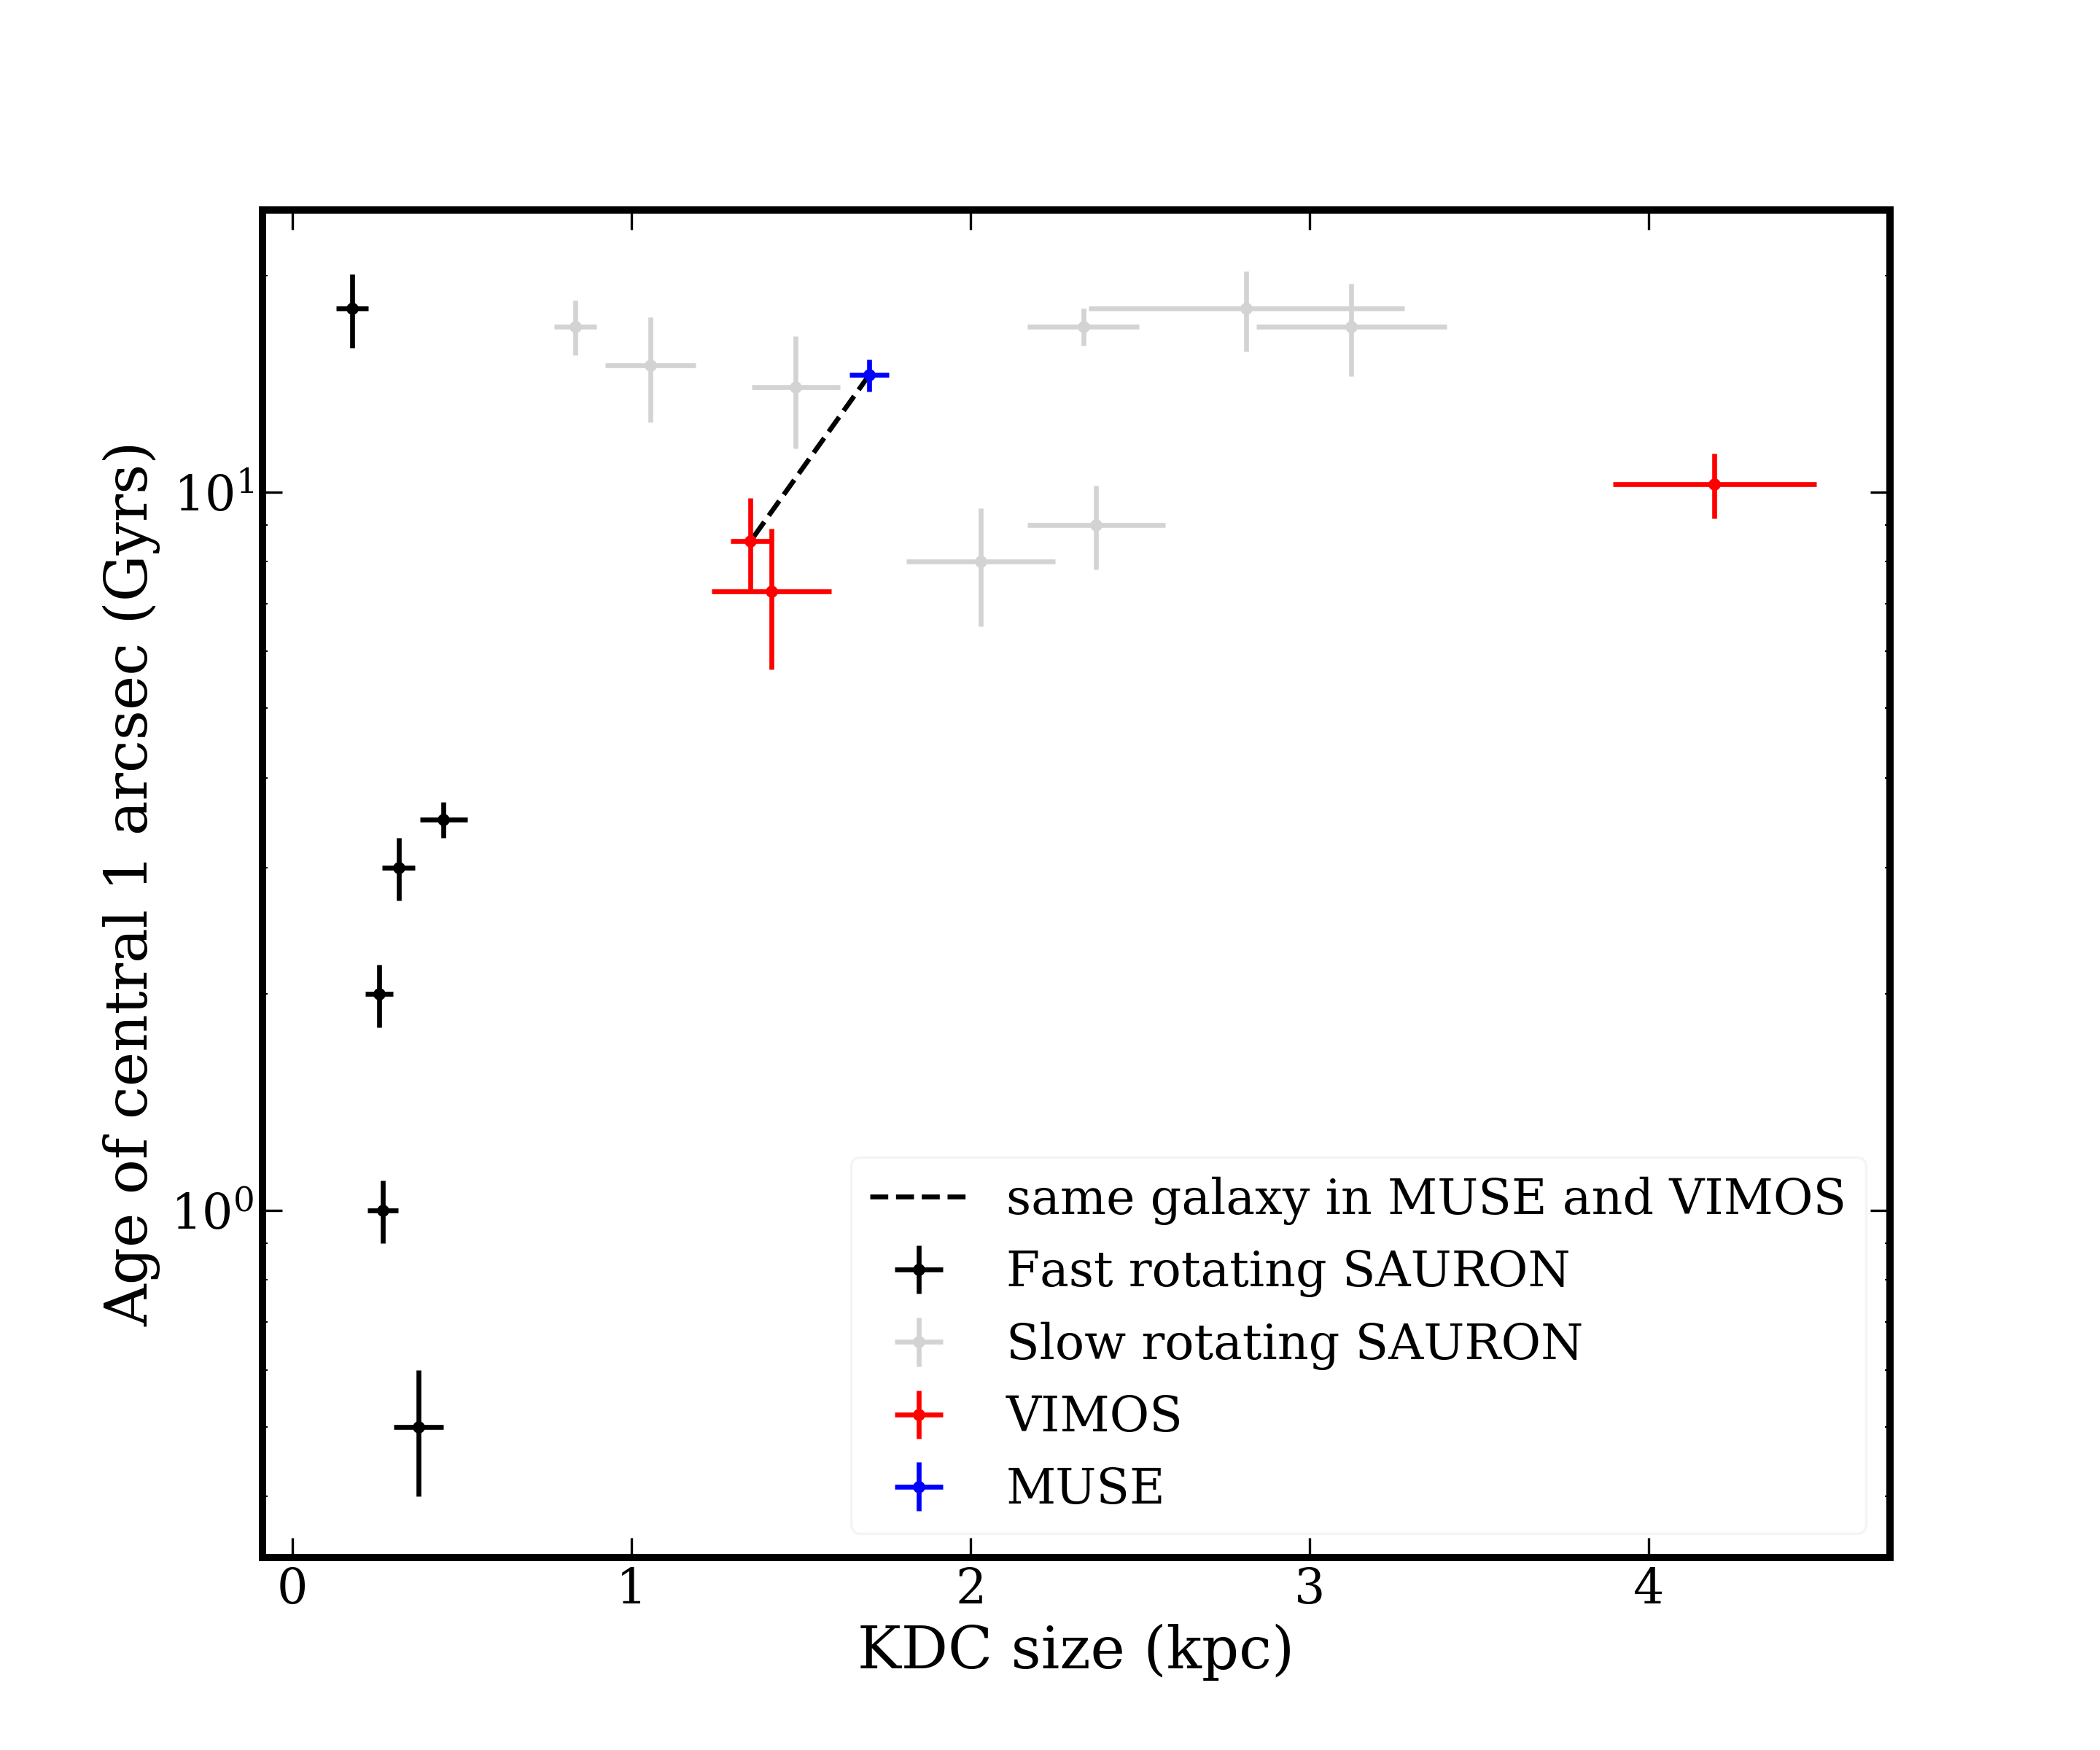
\includegraphics[width=\columnwidth]{KDC_size_age.png}
  \caption[KDC dichotomy]{KDC size\,--\,age relation. KDCs can be
    separated into two classes: old (and potentially large) and
    embedded in a slow rotator or small (and generally young) and
    embedded in a fast rotator. Our Southern Sample VIMOS and MUSE
    measurements are shown in red and blue, respectively, while the
    measurements from SAURON \citep{Kuntschner2010} are shown in black
    and grey for respectively fast and slow rotators. {\bf (In the
      legend, ``same'' should be ``Same'', ``Fast rotating'' should be
      ``Fast-rotating'', and ``Slow rotating'' should be
      ``Slow-rotating''. In the y-axis label, ``Gyrs'' should be
      ``Gyr''.)}}
  \label{fig:KDC}
\end{figure}

\section{Ionised Gas Source}
\label{sec:gas}

\subsection{Ionised Gas Distribution and Mass}
\label{subsec:gas_mass}

Using the methods described in Section~\ref{subsec:EmissionLines}, we
find the best-fitting LOSVD of the emission lines in each bin of our
Southern Sample galaxies. As with the stellar LOSVD, this is assumed
to be Gaussian in shape and is thus parametrised by the mean velocity
and velocity dispersion only. For each detected galaxy, the integrated
flux map in the [\ion{O}{iii}]$\lambda\lambda$4957,5007 doublet is
shown in Appendix~\ref{sec:maps} (we choose to show [\ion{O}{iii}], as
detection of any of the other emission lines first requires a
detection of [\ion{O}{iii}]; see
Section~\ref{subsec:EmissionLines}). When the emission is spatially
extended, we also show the [\ion{O}{iii}] mean velocity and velocity
dispersion maps in Appendix~\ref{sec:maps}.

Only $4$ galaxies (IC~1459, NGC~612, NGC~1316 and NGC~3100) of our
Southern Sample have emission lines detected outside of a central
\removed{region} \added{1--2 spaxels. This means no structure can be
 resolved}. Of the remaining $7$ galaxies, $5$ (IC~1531, IC~4296,
NGC~3557, NGC~7075 and ESO~443-G024) are only detected in their centre
(so only the integrated flux map is shown in Appendix~\ref{sec:maps}),
and $2$ (NGC~1399 and PKS~718-34) have no detection of any emission
line in a spatially-resolved manner (so no ionised gas map is shown in
Appendix~\ref{sec:maps}). For each individual galaxy, all the emission
lines have a similar distribution (but different fluxes). {\bf (It
  would help in this paragraph to define what you mean by
  ``centre''. E.g.\ ``a centred circular region of radius
  $???\arcsec$'' or ``within $???\arcsec$ of the centre. Add.)}

\removed{As can be seen from the maps in Appendix~\ref{sec:maps}, 
both NGC~612 and NGC~3100 have significant off-centred ionised 
gas emission.} {\bf (What do you mean by ``significant'' here? Bright?
  Clarify. Equivalently, why is the off-centred emission in IC~1459
  and NGC~1316 not considered significant?)} 
\added{The ionised gas emission for both NGC~612 ).} In NGC~612, 
the ionised gas does not appear related to either the radio jet 
(extending $\approx200$~kpc to the East and West of the galaxy 
centre) or the CO, but in NGC~3100 the ionised gas is spatially 
coincident with both the radio jet and the gap in the CO ring.

Total ionised gas masses can be derived using the prescription of
\citet{Sarzi2005}. This is a very rough calculation, however, so the
values should not be used for quantitative applications. The approach
follows \citet{Kim1989}, whereby the total mass of \ion{H}{ii}
($M_\text{\ion{H}{ii}}$) is given by
\begin{equation}
  \left(\frac{M_\text{\ion{H}{ii}}}{M_\odot}\right)=280\left(\frac{D}{10\,\mathrm{Mpc}}\right)^2\left(\frac{F(\mathrm{H\alpha})}{10^{-14}\,\mathrm{erg\,s^{-1}\,cm^{-2}}}\right)\left(\frac{10^3\,\mathrm{cm^{-3}}}{n_\mathrm{e}}\right)~,
\end{equation}
where $D$ is the galaxy distance, $F(\mathrm{H\alpha})$ is the
H$\alpha$ flux measured from a spectrum created by spatially
integrating over a central circular aperture of radius
$R_\mathrm{e}/2$ (selected to exclude the noisy outer regions of the
observations, but still include the bulk of the gas in galaxies with
significant spatially-extended emission), and as in \citet{Sarzi2005}
we choose an electron density $n_\mathrm{e}=100$~cm$^{-3}$. This
method assumes an ionised gas temperature of $10^4$~K and case-B
recombination \citep{Kim1989}. Like \citet{Sarzi2005}, we only claim a
detection if the amplitude-to-noise ratio $A/N>4$ for [\ion{O}{iii}]
and $>2.5$ for H$\beta$ (VIMOS data) or H$\alpha$ (MUSE data). When
these two conditions are not met, upper limits are calculated assuming
the gas has $A/N=2.5$ and the same velocity dispersion as the stars.

Our calculated ionised gas masses are listed in
Table~\ref{tab:derivedProp}. They are at the upper \removed{edge} 
\added{range} of, and \removed{possibly} \added{occasionally} exceed, 
{\bf (Why ``possibly''? They either always exceed, generally exceed, 
occasionally exceed, or never exceed! Check and clarify.)} the 
typical masses observed in ETGs 
\citep[e.g.][]{Phillips1986, Zeilinger1996, Sarzi2005}. Given that 
our sample contains particularly massive galaxies, however, 
high ionised gas masses are not unexpected.

\subsection{Ionised Gas Kinematics}
\label{subsec:GasKin}

Maps of the best-fitting ionised gas kinematics (mean velocity and
velocity dispersion), as measured with the methods described in
Section~\ref{subsec:EmissionLines}, are shown in
Appendix~\ref{sec:maps} for the $4$ galaxies with spatially-extended
emission lines (IC~1459, NGC~612, NGC~1316 and NGC~3100). Because gas
is dissipational (contrary to stars), it is expected that given
sufficient time, the ISM will always settle into a disc. The maps in
Appendix~\ref{sec:maps} show that the ionised gas (i.e.\ the warm
component of the ISM) of our Southern Sample galaxies varies from
largely settled discs (IC~1459 and NGC~612) to more disordered
kinematics (NGC~3100) to a possible inflow (NGC~1316).

It is immediately clear when comparing the stellar and ionised gas
mean velocity maps that, where gas is detected, its rotation (or,
equivalently, its projected angular momentum) is often not aligned
with that of the stars. As noted before \citep[e.g.][]{Davis2011a}, a
misalignment between the kinematics of the stars and gas suggests an
external origin for the gas (e.g.\ accretion or wet merger). The
converse is not necessarily true, i.e.\ aligned kinematics is
consistent with an internal origin (e.g.\ stellar-mass loss) but does
\emph{not} require it.

We now comment in turn on the $4$ galaxies with spatially-extended
ionised gas.

{\bf (In the following paragraphs, as all $4$ galaxies are quite
  famous (the first $3$ anyway), you should really quote the past
  literature/papers when you discuss an aspect/feature/property that
  has already been observed/shown/mentioned before, as many of these
  aspects have. So do have a look at the literature on each object.)}

\removed{\textbf{IC~1459} has ionised gas counter-rotating with respect to the
stellar KDC, but it is also misaligned with respect to the outer stars
of the host galaxy (i.e.\ the stars beyond the KDC), that are
non-rotating (see Fig.~\ref{fig:ic1459}). The ionised gas thus appears
to have a third, independent, axis of rotation.} {\bf (I do not
  understand why you state/claim that here. From the map shown, it
  seems pretty clear to me that the stars in the outer parts of the
  galaxy {\em are} rotating (i.e.\ the top-left is red and the
  bottom-right is blue), and that they are rotating in a manner
  consistent with the ionised gas, just as \citet{Franx1988}
  claimed. Convince me otherwise of change your statement!)} \removed{This is
contrary to \citet{Franx1988} who claims that the rotation of the gas
is aligned with that of the stars outside of the KDC. As the stellar
disc did not survive the merger event that created the KDC, }{\bf (How
  do you know there was a stellar disc to start with? Clarify or
  rephrase.)} \removed{it is unlikely that the gas in the progenitor of IC~1459
survived. However, the lost gas may have remained bound and been
re-accreted, so that the gas observed today preserves a fossil record
of the galaxy's original disc. Alternatively, the ISM may have yet
another external origin.}

\added{\textbf{IC~1459} has ionised gas co-rotating with the outer part (not the KDC) of the host galaxy \citep{Franx1988}. Whilst this is consistent with an internal origin of the gas, it should be noted that a major merger is typically expected to deplete a galaxy's gas reservoir. Either this did not happen in this case (a major merger being evidenced by the existence of the KDC) or the ISM may has an external origin and the apparent alignment of the gas and outer stars is random.}

\textbf{NGC~612} has well aligned stellar and ionised gas kinematics
(see Fig.~\ref{fig:ngc612}), the misalignment angle (measured as
described in Section~\ref{subsubsec:KinPA}) being just
$1\fdg0\pm0\fdg7$, thus consistent with an internal gas origin. This
adds to the evidence {\bf (What is the other evidence?
  Summarise/quote it or rephrase.)} that NGC~612 has not undergone a
recent major merger (major mergers exhaust galaxies of their gas and
destroy stellar discs), suggesting in turn that the fuelling of the
radio jet could be a purely secular process.

%**********************************************************************
%This plot no longer exists... Which plot?!
%**********************************************************************

\textbf{NGC~1316} is a complex object. The existence of redshifted
emission lines with respect to the rest frame of the galaxy on both
sides of the galaxy shows the gas is not in a settled disc and there
must be some inflows/outflows. Even from a visual inspection of the
ionised gas velocity field (see Fig.~\ref{fig:ngc1316}), it is clear
that a simple exponential disc model will not fit the data well. We
instead speculate that that the high-velocity peak to the South-West
of the centre is an inflow towards the nucleus, {\bf (Is there any
  evidence for this? If so, state them!)} almost perpendicular to the
radio jet, although other interpretations are possible. Better quality
data (better $S/N$ and a wider field of view) coupled with more
sophisticated models are required to test this interpretation.
% Nevertheless, it is clear that the gas in not in a settled disc.
		
% Without filling in some of the regions were we do not detect
% emission lines through additional observations, it is impossible to
% judge the state or even existence of a disc.

\textbf{NGC~3100} has an interesting ISM morphology. The
\ce{^{12}CO(2-1)} integrated intensity contours (overlaid on the IFS
maps in \removed{white} \added{cyan}; see Fig.~\ref{fig:ngc3100}) 
{\bf (Again, no white
  contours in the figure... pale blue/turquoise contours?)} show a
broken ring, the radio jet passing through the gaps, hence suggesting
a jet-ring interaction \citep[see][]{ruffa2019, ruffa2020}. The
ionised gas is brightest in those same gaps, that we interpret as
additional excitation of the gas due to shocks from the impact of the
jet. It is unclear if the ionised gas kinematics supports this
interpretation, being completely different than that of the stars (and
nearly totally blueshifted). The centre of rotation of the gas also
appears to be offset from the centre of the galaxy (as defined by its
stellar surface brightness), by several arcseconds to the west. {\bf
  (I really do not understand how you can identify a centre of
  rotation when there is no evidence of organised rotation at
  all. Either convince me of that or remove/change that
  comment. Perhaps mention the lack of obvious large-scale rotation
  instead?!)}

\subsubsection{Kinematic Misalignments}
\label{subsec:kinmis}

\citet{Davis2011a} showed that only $36\pm5\%$ of fast rotators have
ionised gas kinematics misaligned with respect to that of the stars,
while slow rotators have a nearly flat distribution of misalignment
angles (see, e.g., Fig.~4 of \citealt{Davis2011a}). This indicates
that the source of ionised gas is primarily external in slow rotators,
while it can be either external or internal in fast rotators. The
observations of our Southern Sample are consistent with this: the only
slow rotator with spatially-extended ionised gas is IC~1459, that has
significantly kinematically-misaligned gas, while of the $3$ fast
rotators with spatially-extended ionised gas, only $1$ (NGC~3100) is
definitely misaligned (the misalignment angle of NGC~612 is consistent
with an internal gas origin while that of NGC~1316 is unclear).
% , although the best-fitting exponential disc model (see Fig.\
% \ref{fig:Inflow}) is definitely misaligned to the stellar
% kinematics.
             
\subsection{Ionisation Sources}
\label{subsec:Diagnostics}

Determining the sources of ionising radiation in galaxies using
emission line ratios, such as Baldwin\,--\,Phillips\,--\,Terlevich
(BPT) plots (\citealt{Baldwin1981}; revised by e.g.\
\citealt{Kewley2001, Kewley2006} and \citealt{Kauffmann2003a}), has
become an increasingly widespread exercise. That said, there are
several important caveats. Firstly, great care must be taken when
applying each diagnostic; much of the literature misinterprets the
resulting classifications. Secondly, in the absence of
spatially-resolved spectra, low-ionisation nuclear emission-line
region (LINER) classifications have often been taken as a marker for
jet-mode AGN. However, several recent surveys have shown that many of
these may not be bona-fide AGN \citep[e.g.][]{Sarzi2005, Sarzi2010,
  Singh2013, Belfiore2016a}. In these cases, the emission may not even
originate exclusively from the galaxy centres, the location of the
putative AGN. This led to the creation of the low-ionisation
emission-line region (LIER) classification, with the same criteria as
LINERs, but not necessarily restricted to the nuclear regions.

The challenge to classify ETGs using emission line ratios is that they
often have very little ionised gas and weak ionising radiation fields,
so that it is often difficult to detect emission lines from their
ISM. In addition, the BPT plots require spectral lines spread over a
wider spectral range than many IFSs deliver. This has given rise to a
number of other, analogous, classification criteria and plots, that we
take advantage of here. A description of our ionisation source
classification process thus follows below.

First, we preferentially use the original BPT plots for the galaxies
observed with MUSE, that has the required spectral range. This allows
us to classify galaxies into the star-forming, LINER/LIER or Seyfert~2
class. For the emission line fluxes derived from VIMOS data, we use
the [\ion{N}{i}]/H$\beta$ versus [\ion{O}{iii}]/H$\beta$ plot of
\citeauthor{Sarzi2010} (\citeyear{Sarzi2010}; hereafter the SAURON
plot). Unlike the BPT plots, \citet{Sarzi2010} does not define
classification boundaries. Using Eq.~\ref{eq:N_dec}, we thus transform
the [\ion{N}{ii}]/H$\alpha$ BPT plot classification boundaries of
\citet{Kewley2001} and \citet{Kauffmann2003a} to the
[\ion{N}{i}]/H$\beta$ SAURON plot. This allows us to classify those
galaxies into the star-forming or LINER/Seyfert~2 class. We also use
the so-called WHaN2 plot (H$\alpha$ equivalent width versus
[\ion{N}{ii}]/H$\alpha$) from \citet{CidFernandes2011}. Using
Eqs.~\ref{eq:EqW_dec} and \ref{eq:N_dec}, we transform their boundary
lines into an H$\beta$ equivalent width versus [\ion{N}{i}]/H$\beta$
(WHbN1) plot for the VIMOS data. This allows us to classify those
galaxies into the star-forming, strong AGN (Seyfert~2), weak AGN
(LINER) or retired class.

To check if the LINER classifications are due to central radiation
sources (such as AGN) or extended sources (such as weak star formation
or stars on the post-asymptotic giant branch, pAGB), {\bf (What about
  extended horizontal branch stars (again below)? Mention/discuss.)}
we examine the H$\alpha$ and H$\beta$ flux radial profiles of our
Southern Sample galaxies with extended detected ionised gas (see
Section~\ref{subsubsec:Hb}). Finally, we use the mass\,--\,excitation
(MEx) plot of \cite{Nyland2016}, using parameters derived from \added{a} 
spectra \added{produced by} spatially-\removed{integrated}\added{integrating} over \added{a} central circular apertures of radius
$3\arcsec$ \added{to probe} \removed{, thus probing only} the central 
regions of the galaxies (see
Section~\ref{subsubsec:MEx}). {\bf (You talked here of *the*
  spatially-integrated spectra, as if spectra within a central
  $3\arcsec$ aperture had been used before, but this is not the case
  (only $2\arcsec$ and $1\arcsec$ apertures were used for stellar
  populations). Are these new or previously-generated spectra?
  Clarify.)} This allows us to classify the remaining galaxies (with
no spatially-extended ionised gas) into the star-forming, Seyfert~2,
LINER, transition or passive class, and to subdivide LINER galaxies
into those whose LINER characteristics are attributable to a central
AGN (labelled as LINER-AGN) and those whose LINER characteristics are
not \added{(simply labelled as LINER: they may be AGN or LIER)}. 
{\bf (Labelled as what? LIER?  Clarify.)} As the least
conventional, we expand on the final two steps in the two sub-sections
below, while the final classifications are listed in~Table
\ref{tab:derivedProp}.

% \subsection{BPT Diagnostics}
% \label{subsec:BPT}
% Firstly, in Fig.\,\ref{fig:BPT}, we examine our galaxies using the
% classic BPT diagnostic plots. For the plots using
% [\ion{N}{ii}]/H$\alpha$, [\ion{S}{ii}]/H$\alpha$ and
% [\ion{O}{i}]/H$\alpha$ versus [\ion{O}{iii}]/H$\beta$, we can only
% use the emission-line fluxes derived from our MUSE datacubes, as the
% lines necessary for gauging the hardness of the ionising radiation
% field are outside the spectral range of VIMOS. Only two MUSE
% galaxies have detections of the necessary emission lines: IC~1459
% and NGC~1316. Both occupy very similar positions in the BPT plots,
% on or close to the boundary between the Seyfert 2 and LINER
% classes. On the whole, the central bins tend to be on the LINER
% side.

% \begin{figure}
%   \centering
%   \includegraphics[width=.9\textwidth]{chapter5/BPT.png}
%   \caption[BPT plots]{BPT plots for IC~1459 and NGC~1316. The colour
%   scale (blue to yellow) represents increasing distance from the
%   galaxy centre. The classification boundaries are from
%   \citet{Kewley2006}.\label{fig:BPT}}
% \end{figure}

% \begin{figure}
%   \centering
%   \includegraphics[width=0.7\textwidth]{chapter5/SAURON.png}
%   \caption[An alternative diagnostic plot]{SAURON diagnostic plot
%   for the line ratios available in the VIMOS datacubes. To show the
%   expected position of LINERs on the SAURON plot, the MAPPINGS-III
%   shock model grid of \citet{Allen2008} is shown in green. The solid
%   lines are lines of constant shock velocity (from 150 to
%   1000\,$\mathrm{km\,s^{-1}}$) and the dotted lines are lines of
%   constant magnetic parameter $b \equiv B/\sqrt{n}$ (from 0.5 to
%   4.0), where $B$ is the magnetic field strength and $N$ the
%   (pre-shock) particle number density \citep{Dopita1996}. All models
%   assume an electron density of
%   $n_\mathrm{e} = 1\,\mathrm{cm^{-3}}$.\label{fig:SAURON}}
% \end{figure}

% \citet{Sarzi2010} showed that Seyferts, LINERs and star-forming
% galaxies are reasonable separated in the SAURON diagnostic plot. To
% exploit the VIMOS datacubes we thus use the
% [\ion{N}{ii}]\,--\,[\ion{N}{i}] relation derived in Section
% \ref{subsec:Ndec}, along with the Balmer decrement, to transform the
% \citet{Kewley2001} extreme starburst and the \citet{Kauffmann2003a}
% pure star-formation boundaries in the [\ion{N}{ii}]/H$\alpha$ versus
% [\ion{O}{iii}]/H$\beta$ plot to boundaries in the SAURON plot. For
% the MUSE datacubes, only IC~1459 and NGC~1316 have detections of
% [\ion{N}{i}]. Given that we already have the superior classic BPT
% plots for these galaxies, we only show the VIMOS-derived SAURON
% diagnostic plot. This is shown in Fig.\,\ref{fig:SAURON} for all 6
% VIMOS galaxies with detectable, spatially-resolved emission
% lines. All exhibit LINER-AGN behaviour.

% NGC~3100 appears to occupy to distinct regions in the SAURON
% diagnostic plot (Fig.\ \ref{fig:SAURON}). If the ionisation is due
% to shocks from the impact of the jet, then using the shock models of
% \citet{Allen2008}, we can see that the right-hand group of bins have
% been ionised by a higher shock velocity that the left-hand group. As
% can be seen in Fig.\ \ref{fig:ngc3100_NI_Hb}, these bins are
% directly in the gap (presumable created by the jet blowing a hole)
% in the CO ring.

% \begin{figure}
%   \centering
%   \includegraphics[width=0.5\textwidth]{chapter5/vimos/ngc3100_NI_Hb.png}
%   \caption[NGC~3100 \bracket{\ion{N}{i}}/H$\beta$ line ratio
%   map]{The [\ion{N}{i}]/H$\beta$ line ratio map of NGC~3100, showing
%   the hardest ionisation field is in gap in the CO ring (white
%   contours), spatially coincident with the radio jet (green
%   contours). Surface brightness contours are in black.}
%   \label{fig:ngc3100_NI_Hb}
% \end{figure}
	 
% \subsection{WHaN2 Plots}
% \label{subsec:WHaN2}

% \begin{figure}
%   \centering
%   \includegraphics[width=0.8\textwidth]{chapter5/WHaN2.png}
%   \caption[WHaN2 plot for IC~4296]{WHaN2 plot for IC~4296. The
%   colour scale (blue to yellow) represents increasing distance from
%   the galaxy centre.}
%   \label{fig:WHaN2}
% \end{figure}

% \begin{figure}
%   \centering
%   \includegraphics[width=0.8\textwidth]{chapter5/WHbN1.png}
%   \caption[VIMOS WHbN1 plot]{VIMOS WHbN1 plot. All galaxies have
%   decreasing H$\beta$ emission with increasing distance from the
%   galaxy centre.}
%   \label{fig:WHbN1}
% \end{figure}

% The final spatially-resolved line ratio diagnostic plot that we use
% is that of the equivalent width of H$\alpha$ versus
% $\log([\text{\ion{N}{ii}}]/H\alpha)$, known as the WHaN2 plot
% \citep{CidFernandes2011}. We interpret the strong AGN, weak AGN and
% retired regions on this plot as Seyfert 2, LINER-AGN and LIER
% classifications, respectively. Passive (i.e.\ line-less) galaxies
% are marked with crosses instead of circles. Fig.\,\ref{fig:WHaN2}
% shows the WHaN2 plot for the MUSE derived emission lines of IC~4296
% where almost all the bins fall within the weak AGN (LINER-AGN)
% class. This is consistent with the measurements from the VIMOS
% observations of the IC~4296 as shown in the SAURON diagnostic plot,
% where IC~4296 is well within the shocks grid (i.e.\ LINERs; see
% Fig.\ \ref{fig:SAURON}). We do not include IC~1459 and NGC~1316, as
% they have already been classified via the classic BPT plots (see
% Section \ref{subsec:BPT}).

% For the emission lines measured from the VIMOS datacubes, we use
% H$\beta$ as a proxy for H$\alpha$ and [\ion{N}{i}] as a proxy for
% [\ion{N}{ii}] utilising the relations found in Section
% \ref{subsec:Ndec} to transform the classification boundaries (see
% Section \ref{subsec:Ndec}). We call the resulting diagnostic plot
% the WHbN1 plot, shown in Fig.\,\ref{fig:WHbN1}. While in Section
% \ref{subsec:BPT} (Fig.\,\ref{fig:SAURON}) we showed that most of
% these galaxies had line ratios consistent with being ionised by
% shocks such as in LINER-like galaxies, Fig.\,\ref{fig:WHbN1} shows
% that for IC~1459 and NGC~3100, the ionising photons originate from
% the AGN.

\subsubsection{H$\alpha$ and H$\beta$ Radial Profiles}
\label{subsubsec:Hb}

As discussed above, many galaxies traditionally classified as LINERs
are in fact LIERs \citep[see e.g.][]{Sarzi2005, Sarzi2010, Singh2013,
  Belfiore2016}, i.e.\ the source of the ionising radiation is not
concentrated nor limited to the nuclear regions of the galaxies. To
check if the ionising radiation is entirely due to AGN in our Southern
Sample galaxies, we plot the H$\alpha$ (H$\beta$) flux radial profiles
of the MUSE (VIMOS) galaxies in Fig.~\ref{fig:Ha_profile_MUSE}
(Fig.~\ref{fig:Hb_profile_VIMOS}). A point source, such as an AGN,
will result in a radial profile proportional to $r^{-2}$ (and
convolved with the point-spread function, PSF), where $r$ is the
distance of the gas from the galaxy centre. Although the observed
profiles (i.e.\ the bins) are projected on to the sky, a significantly
shallower profile suggests a spatially-extended source, presumably
non-circumnuclear stellar processes such as star formation or
radiation from pAGB stars {\bf (Again.)}, as the dominant cause of the
ionisation in the outer parts of the galaxy (i.e.\ a LIER rather than
a LINER).

\begin{figure}
  \centering 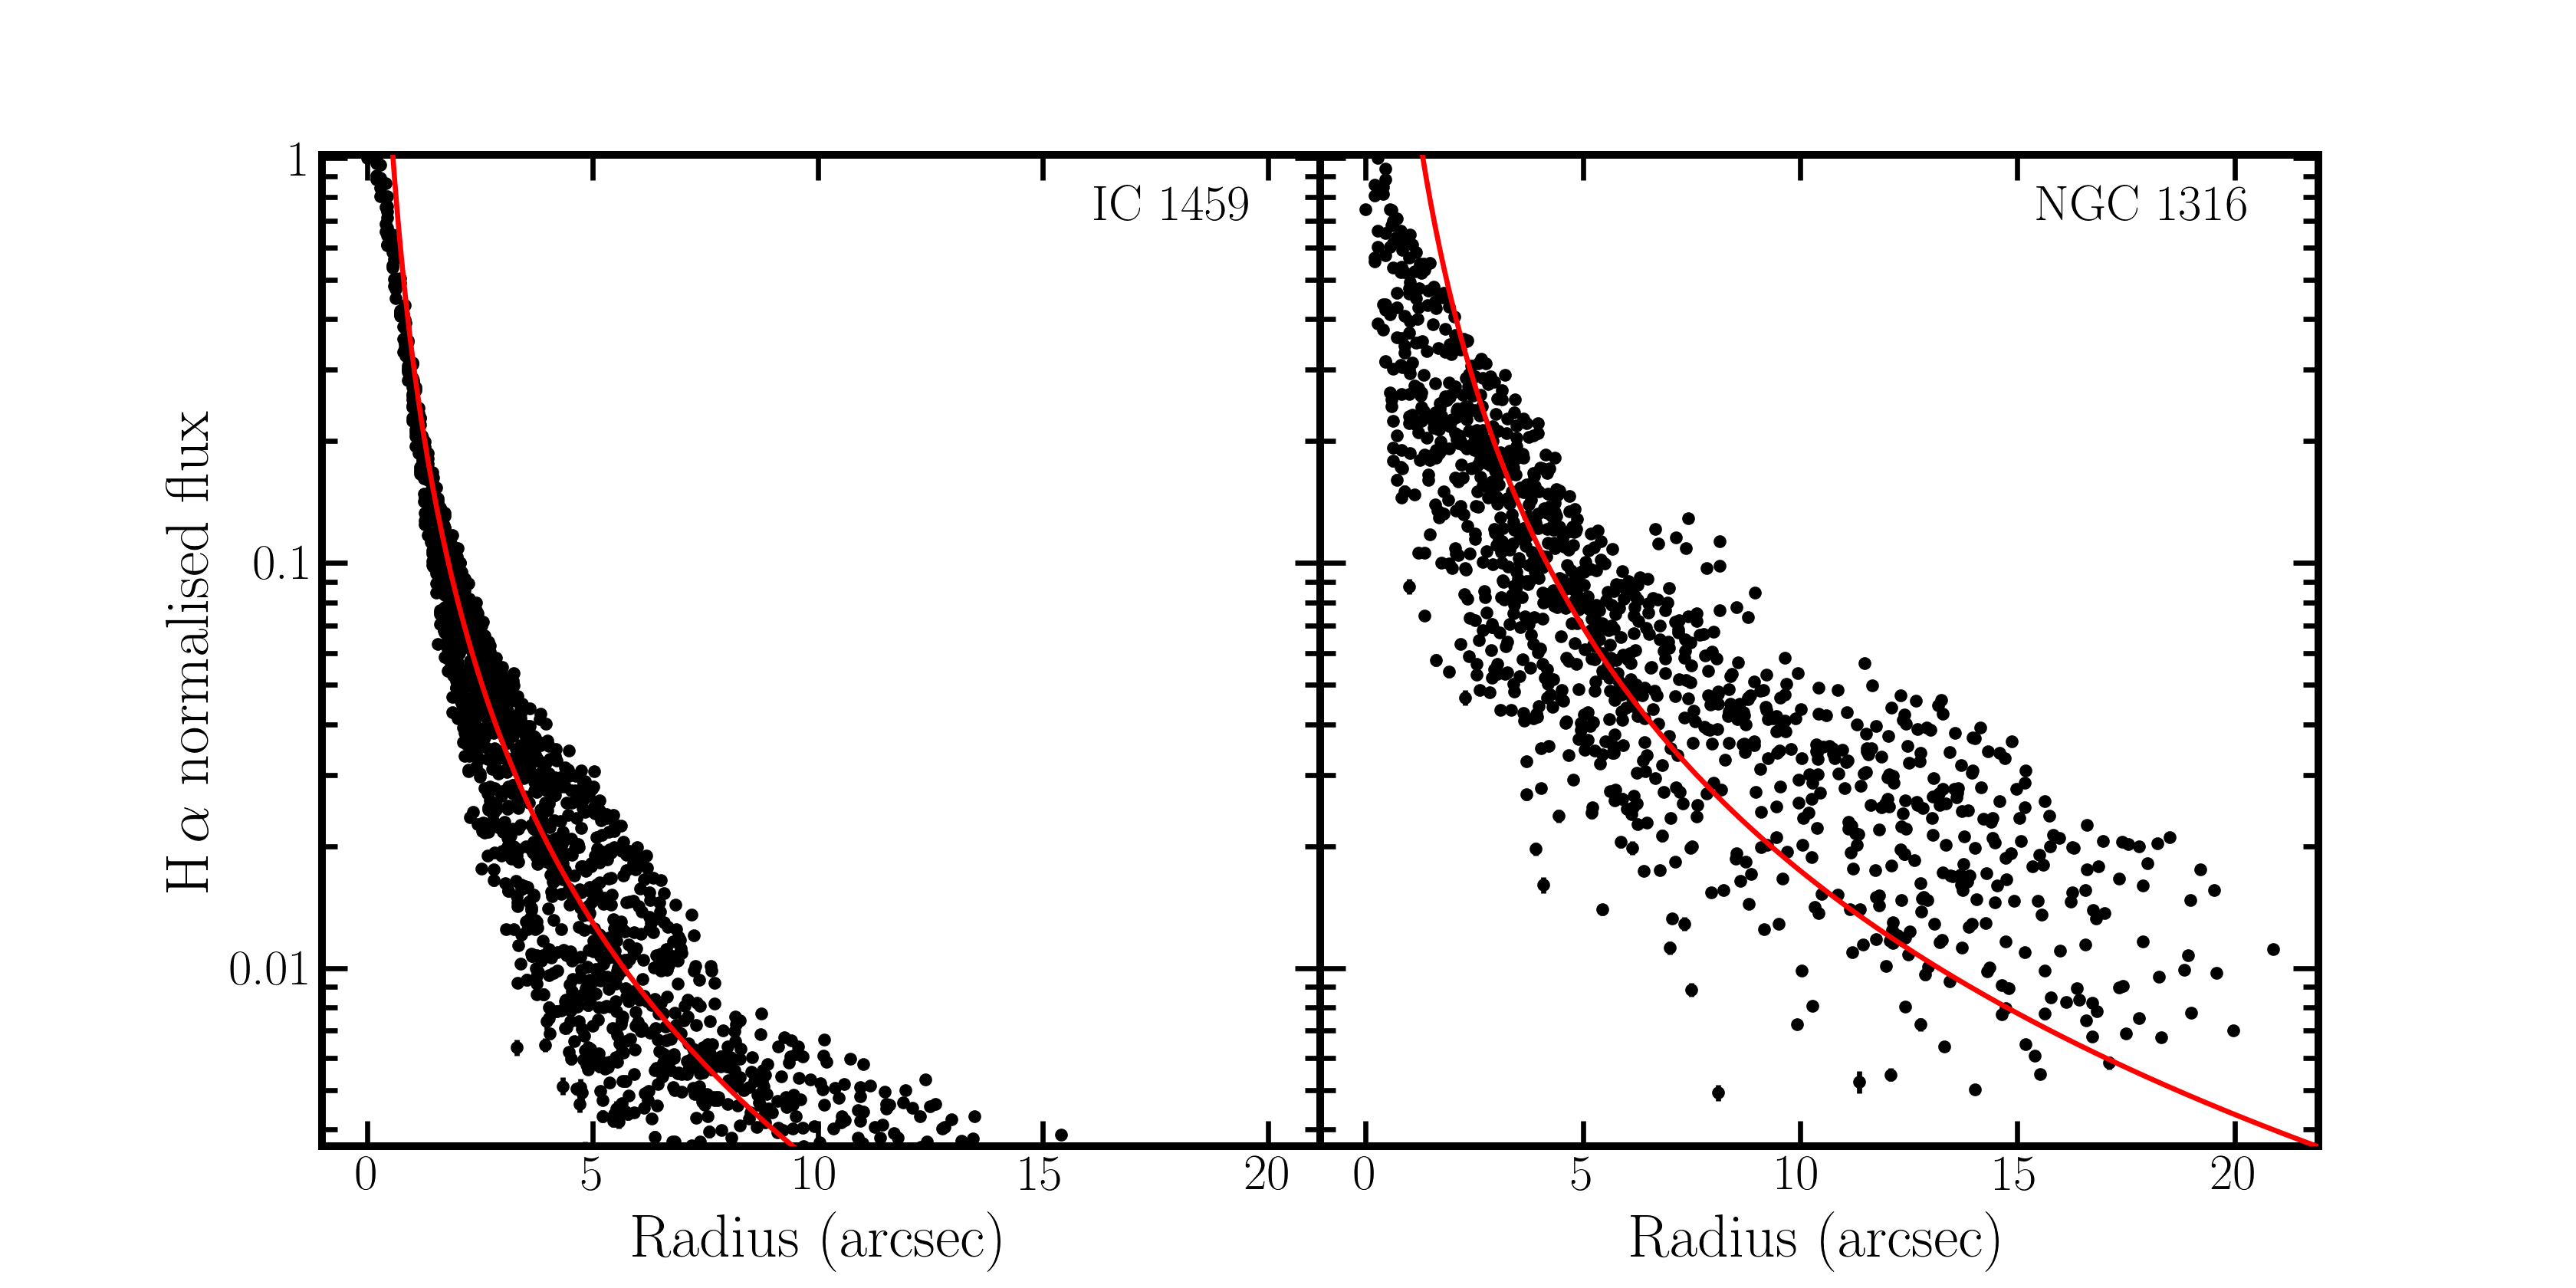
\includegraphics[width=\columnwidth]{Halpha_profile.png}
  \caption{H$\alpha$ flux radial profiles derived from the MUSE
    data. Solid red lines show radial profiles proportional to
    $r^{-2}$, convolved with a Gaussian of width equal to the measured
    PSF. \added{The fitting of these lines was done by eye.}{\bf (But what about the zero-points of the red profiles? How
      are these set? Explain.)} {\bf (Make the axis labels and galaxy
      names as thick as the plot boxes.) {\bf (All labels are rather
        small. Enlarge?)} {\bf (Note that the bounding boxes of
        Figs.~5 and 6 are really bad (much too big), so that the
        ``width='' commands are useless. Please make sure {\em all}
        your bounding boxes are as tight as possible around the
        figures themselves.)}}
    \label{fig:Ha_profile_MUSE}}
\end{figure}

\begin{figure}
  \centering
  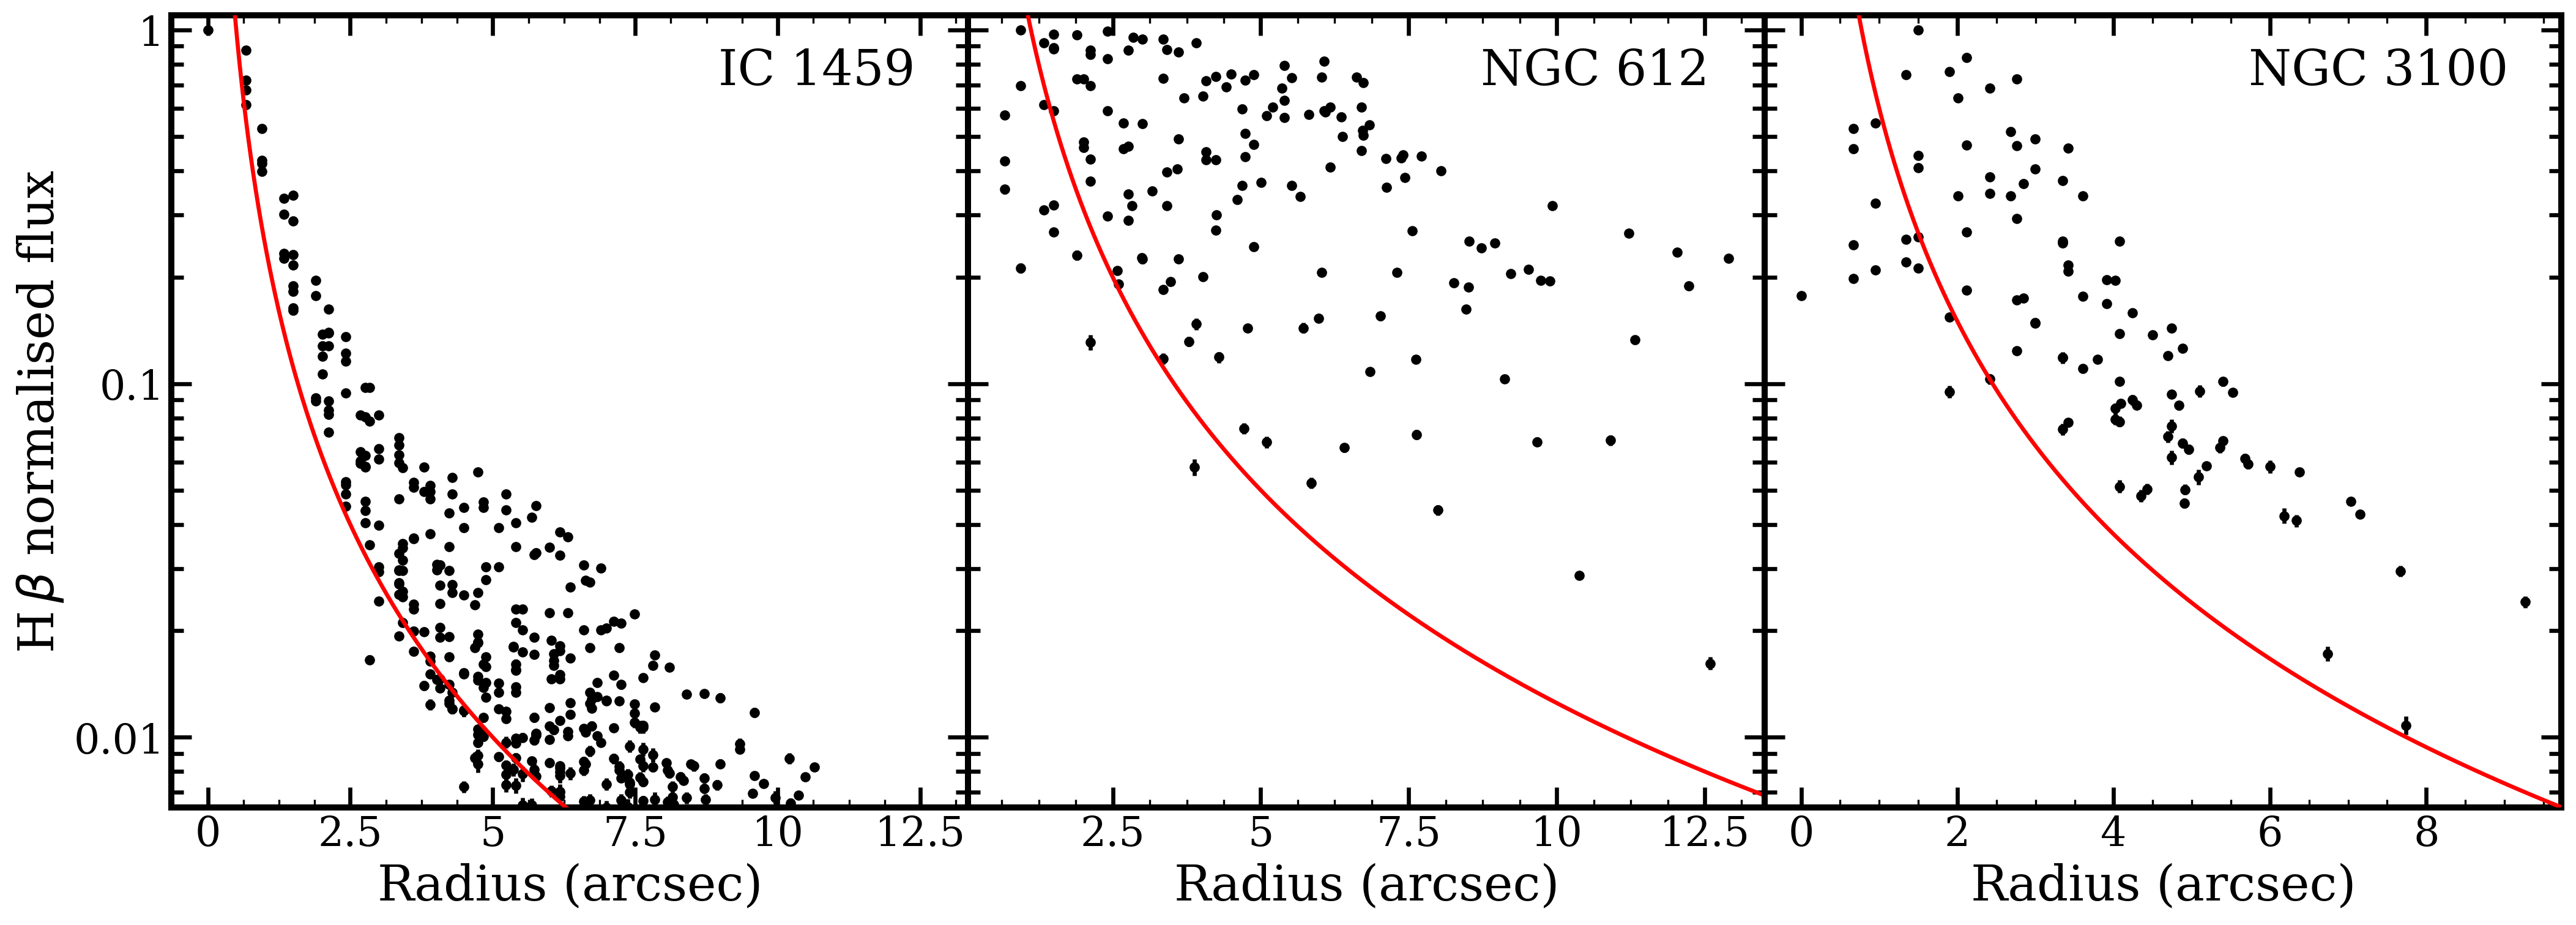
\includegraphics[width=\columnwidth]{Hbeta_profile.png}
  \caption{As Fig.~\ref{fig:Ha_profile_MUSE}, but for the H$\beta$
    flux radial profiles derived from the VIMOS data. {\bf (Make the
      axis labels and galaxy names as thick as the plot boxes.) {\bf
        (All labels are rather small. Enlarge?)}}
    \label{fig:Hb_profile_VIMOS}}
\end{figure}

The radial profiles shown in Figs.~\ref{fig:Ha_profile_MUSE} and
\ref{fig:Hb_profile_VIMOS} suggest that all the galaxies with
spatially-extended Balmer emission in our Southern Sample have a
central point source as the dominant source of the ionising
photons. The H$\beta$ profile of NGC~612 has a larger scatter,
suggesting that stellar processes also have some impact (likely
radiation from pAGB stars {\bf (Again.)}, as NGC~612 has a low
star-formation rate). {\bf (Check what the SFR of NGC~612 actually is,
  to confirm your suspicion, e.g.\ from non-nuclear radio continuum or
  MIR/FIR emission. This may already be discussed in Ilaria's
  papers.)}

\subsubsection{MEx Diagnostic Plots}
\label{subsubsec:MEx}

The mass\,--\,excitation (MEx) plot of \citet{Juneau2011} is useful to
classify galaxies with intermediate excitation levels
($0.5<\mathrm{[\ion{O}{iii}]/H\beta}<8.0$), particularly as it does
not depend on faint lines such as the [\ion{N}{i}] doublet. We use
here the calibrations by \citet{Nyland2016}, including an attempt to
separate LINERs powered by AGN from those powered by pAGB stars (i.e.\
LIERs, with [\ion{O}{iii}] equivalent widths $>0.8$~\AA). We again
focus on the nuclear regions, using a central circular aperture of
radius $3\arcsec$ for all our Southern Sample galaxies. The resulting
diagnostic plot is shown in Fig.~\ref{fig:MEx}.

\begin{figure}
  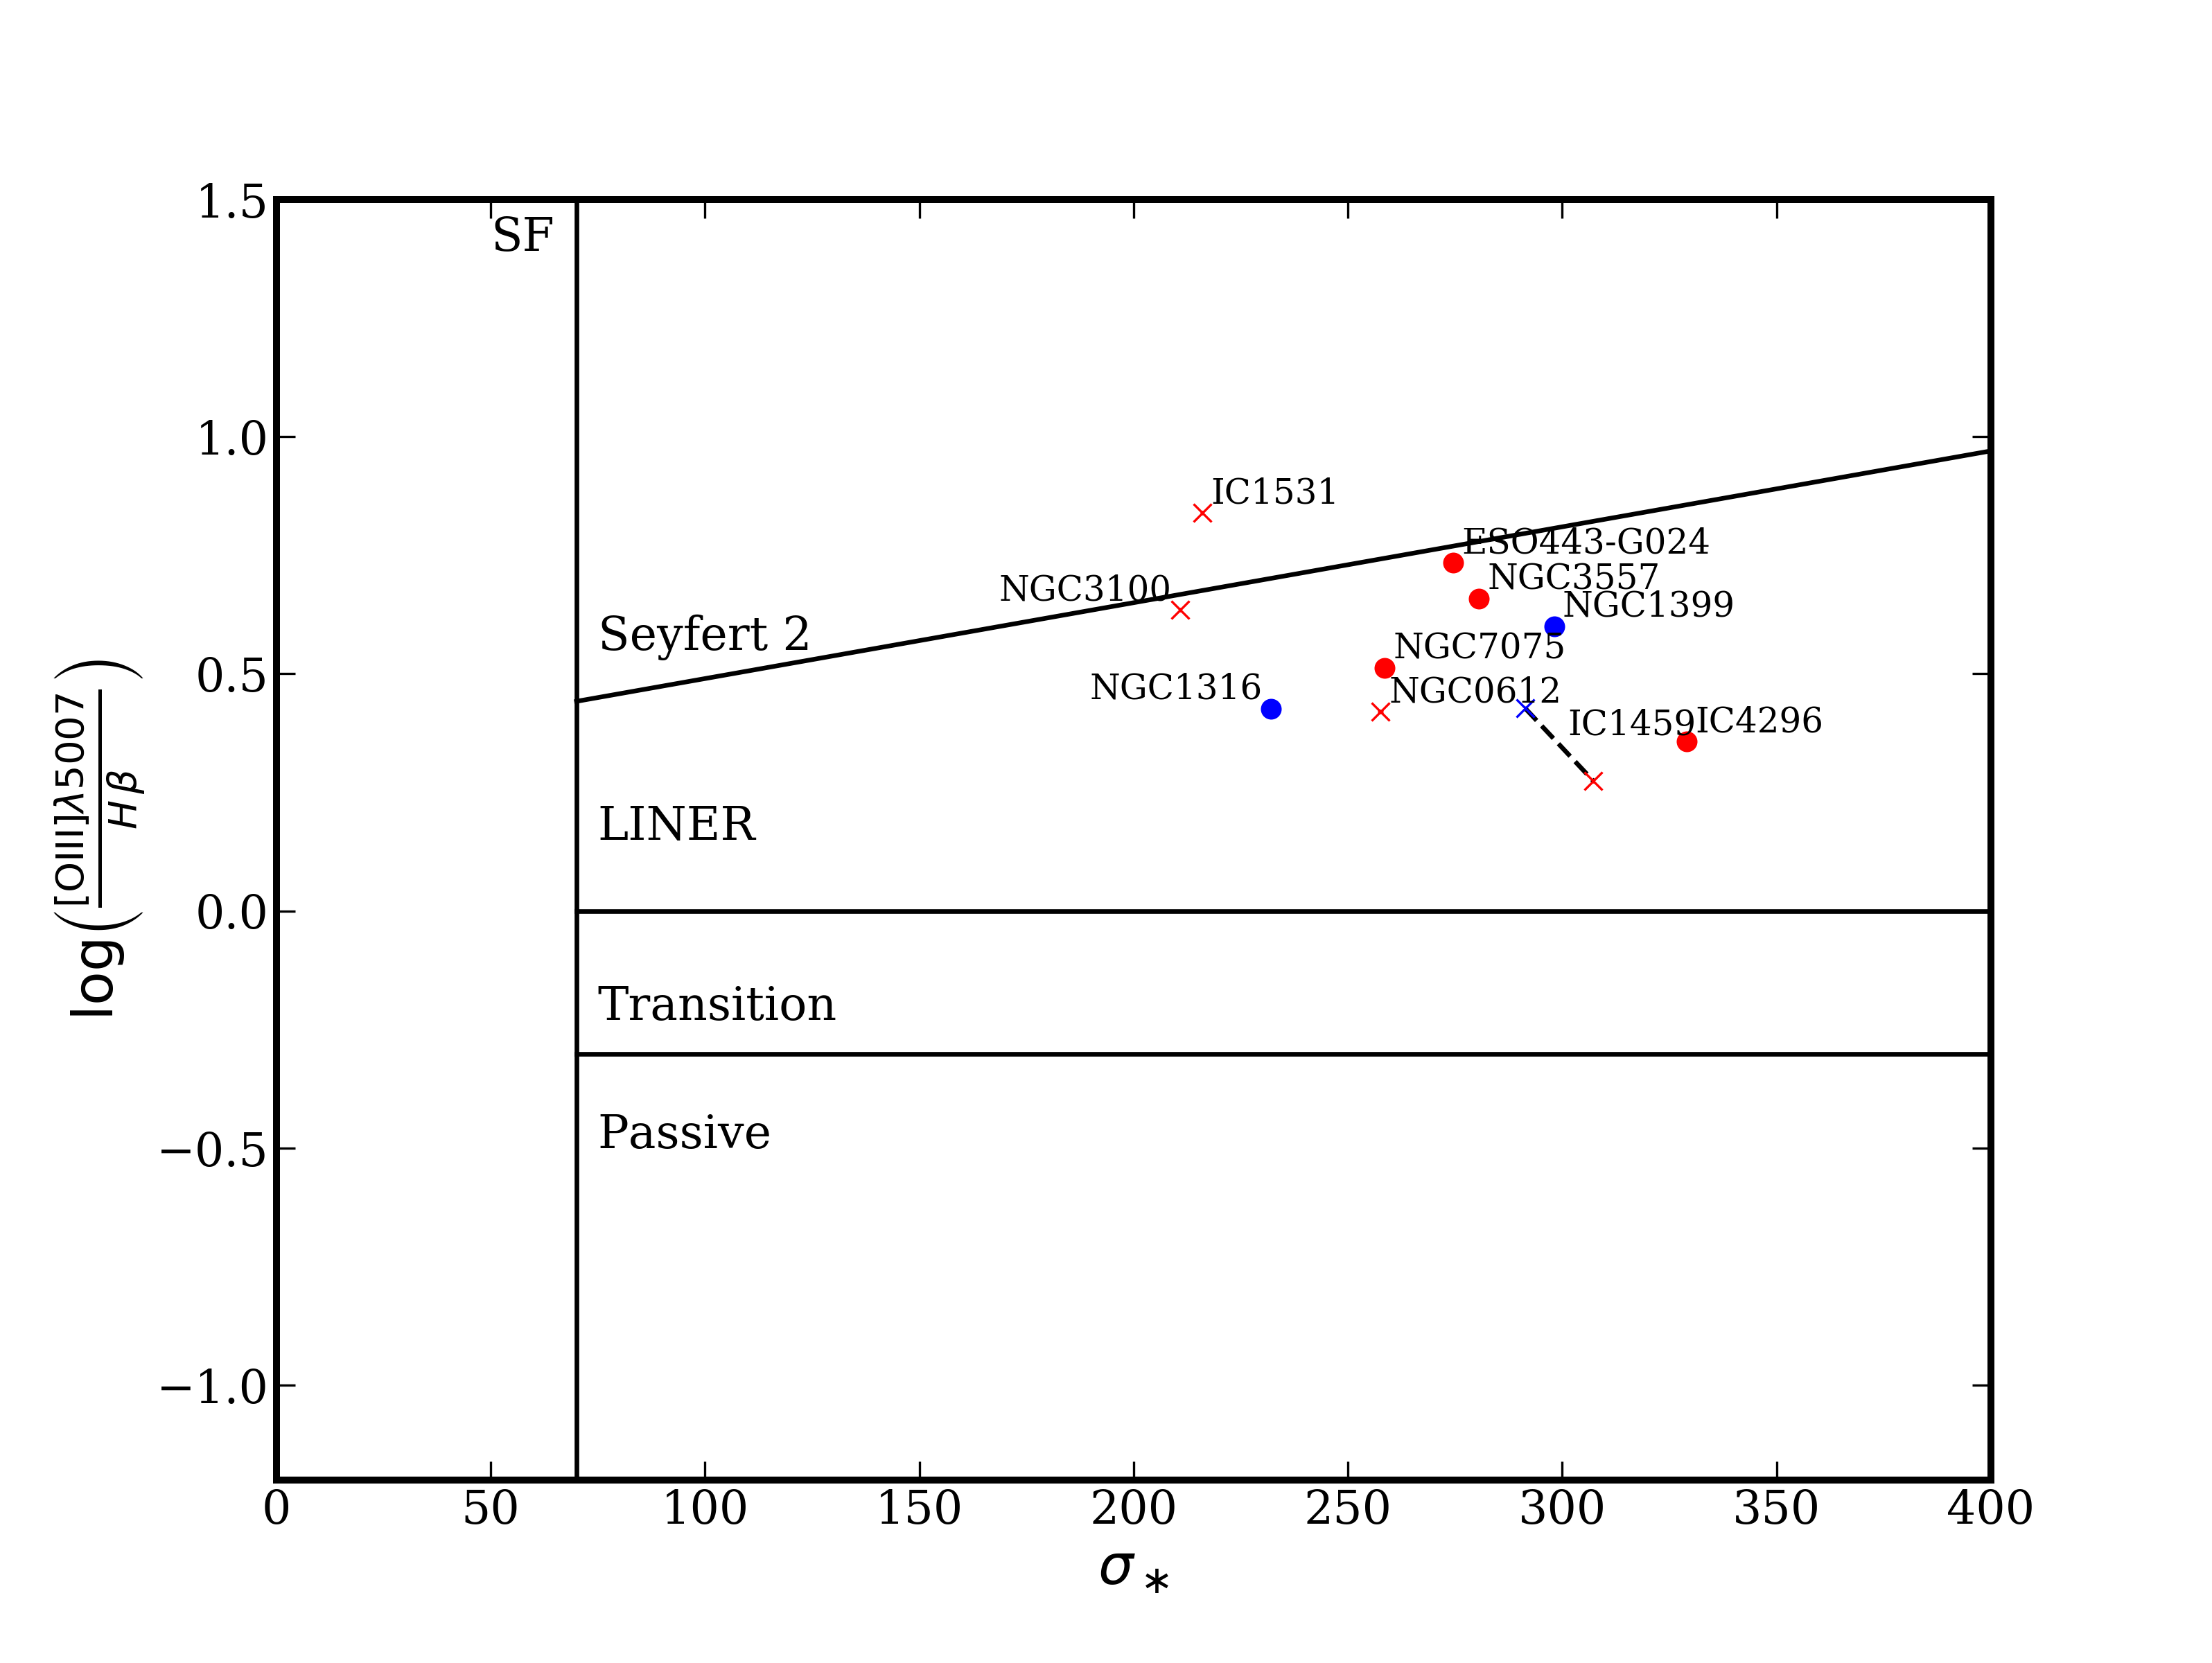
\includegraphics[width=\columnwidth]{nuclear_MEx.png}
  \caption{Nuclear MEx plot, allowing to classify the sources of
    ionising radiation within the central $3\arcsec$ of our Souther
    Sample galaxies. Measurements derived from VIMOS and MUSE data are
    show in red and blue, respectively. Crosses mark galaxies with an
    [\ion{O}{iii}]$\lambda$5007 equivalent width $>0.8$~\AA, while
    filled circles mark galaxies with an [\ion{O}{iii}]$\lambda$5007
    equivalent width $\leqslant 0.8$~\AA. The VIMOS and MUSE
    measurements of IC~1459 are linked by a black dashed
    line. Classification boundaries are from \citet{Nyland2016}. {\bf
      (Use larger data points.)} {\bf (Small ``f'' in ``Star-Forming''
      label. Also add ``(km s$^{-1}$)'' to the x-axis label.)} {\bf
      (All labels are rather small. Enlarge?)}}
  \label{fig:MEx}
\end{figure}

\section{Discussion and Conclusions}
\label{sec:discuss}

In Section~\ref{sec:StarKine}, we showed that in terms of their
stellar kinematic properties our radio-selected Southern Sample
galaxies are no different than ordinary optically-selected ETGs, i.e.\
our sample shows a mixture of regularly- and non-regularly-rotating
objects. \removed{Both classes also appear consistent with observations of the
intrinsic shapes of ordinary regular and non-regular rotators.} {\bf (I
  do not actually know/understand what you were trying to say or refer
  to in the last sentence. Are you referring to the misalignment angle
  $\Gamma_\text{kin}$ of regular and non-regular rotators? What do you
  mean by ``observations of the intrinsic shapes''? Clarify.)} We
established that two (tentatively three) galaxies host a large KDC. We
also classified our sample galaxies into fast- and slow-rotators and,
once differences in the mass distributions of our Southern Sample and
the A+M sample were taken into account, we found a fraction of
slow-rotators ($45\pm13\%$) consistent with that of ordinary ETGs.

\removed{Radio-loud S0 galaxies are extremely rare, with only a handful of
known cases \citep[e.g.][]{Heckman1982, Morganti2011}. This is
presumably due to the mass functions of S0s and radio galaxies,
massive S0s and low-mass radio galaxies both being rare, with similar
transition masses from rare to more numerous. NGC~612 is one of those
rare cases.} {\bf (You are not discussing here any of your own results,
  just rehashing old knowledge, so unless you have something else to
  say about NGC~612 (from your own work), I would suggest to remove
  this paragraph entirely (and/or certainly move it somewhere else
  more relevant).)}

In terms of absorption line strengths and stellar populations
(Sections~\ref{sec:absorption} and \ref{sec:stellarPop}), we found for
our Southern Sample galaxies a gradient of the central Mg~$b$ line
strength versus stellar velocity dispersion relation remarkably
similar to that of \citet{Ziegler1997}. Most of the galaxies in our
Southern Sample have typical ETG properties, with old, metal-rich
stellar populations. {\bf (What about $\alpha$-elements? You should
  also summarise those results here.)} The few exceptions are NGC~612
and NGC~1316, that are both significantly younger than most ETGs, and
NGC~3557, that has a young core. All $3$ KDCs contain old stellar
populations, and they are consistent with being merger remnants. The
KDCs found in Section~\ref{sec:StarKine} are also in agreement with
the KDC age\,--\,size relation found by \added{\citet{McDermid2006}} 
\removed{\citet{Kuntschner2010}} in optically-selected ETGs (see 
Section~\ref{subsec:popKDC}). {\bf (See my previous comment about 
McDermid et al.\ 2006, and perhaps quote it here instead or 
additionally.)}

If cold (e.g.\ molecular) gas is accreted on to the central black
holes of our Southern Sample galaxies to power their nuclear
activities, then unless it is accreted in a highly turbulent fashion
some of it should form stars within the accretion discs
\citep[e.g.][]{Collin1999, Diamond-Stanic2012, LaMassa2013}. If this
is indeed the case, and these young stellar populations are bright
enough to dominate the light, then they should stand out in the
central few spaxels. However, detection of such populations could
prove difficult due to contamination from the AGN continua, the
presence of dust (see Table~\ref{tab:sample} for a description of the
dust morphologies of our Southern Sample galaxies) and the rapid rate
at which a young stellar population fades. In fact, our best-fitting
age maps show no evidence of an abnormally young central stellar
population in any of our galaxies. This is consistent with the results
of other authors such as \citet{GonzalezDelgado2004} and
\citet{Sarzi2005b} with \textit{Hubble Space Telescope} (\textit{HST})
spectra and \citet{CidFernandes2004} with ground-based spectra. In
addition, in Section~\ref{subsec:Diagnostics}, we showed that there is
no evidence of an extended ionising source consistent with ongoing
star formation in any of our targets. {\bf (It seems to me that this
  paragraph is missing a short ``conclusion''. Add one... no evidence
  of any ongoing SF in any of our galaxies?)}

In Section~\ref{sec:gas}, we showed that our Southern Sample galaxies
have ionised gas masses of $10^4$\,--\,$10^6$~$\mathrm{M_\odot}$. As
our sample contains particularly massive galaxies, high ionised gas
masses are not unexpected, but these masses are at the upper limit of,
and \removed{possibly} \added{occasionally} exceed {\bf (Again, why ``possibly''? They either always
  exceed, generally exceed, occasionally exceed, or never exceed!
  Check and clarify.)}, the typical masses observed in ETGs,

The only slow rotator with detected spatially-extended ionised gas,
IC~1459, has a substantial gas\,--\,star misalignment. Its gas thus
likely has an external origin, although it is possible that it has
been re-accreted after it was first ejected during the merger that
created the stellar KDC. Of the other $3$ galaxies with detected,
spatially-extended ionised gas (NGC~612, NGC~1316 and NGC~3100, all
fast rotators), we find that one (NGC~3100) again has kinematic
evidence of an external gas origin, another (NGC~612) is consistent
with an internal origin, while the situation for the third (NGC~1316)
is unclear (although the ionised gas is definitely not in a settled
disc). This is consistent with the findings of \citet{Davis2011a}, who
showed that $36\pm5\%$ of fast rotators have ionised gas kinematics
misaligned with respect to that of the stars, while slow rotators have
a flat distribution of misalignment angles. This indicates that the
source of the gas in slow rotators is predominately external, while it
can be either internal or external in fast rotators.

All galaxies with detected emission lines in our Southern Sample show
line ratios characteristic of LINER or Seyfert~2 galaxies. In
particular, we classify $9$ of our $11$ galaxies as LINERs, and we can
conclusively attribute the ionising photons to the central AGN in $5$
of those. The only Seyfert~2 is the fast rotator IC~1531. This is
consistent with the results of \citet{Nyland2016}, who showed that all
Atlas$^\text{3D}$ ETGs classified as Seyferts are also fast rotators.
The final galaxy, PKS~718-34, has no emission line detection (i.e.\ it
is classified as passive). {\bf (These statistics do not match those
  in paragraph 2 of Sub-section~8.1, where only $9$ galaxies are said
  to be detected in ionised gas (rather than $10$ as inferred
  here). The culprit seems to be NGC~1399, which is listed as
  non-detected in Sub-section~8.1 and Appendix~A, has no emission line
  map in Appendix~B, but is nevertheless classified as a LINER in
  Table~4... how is this possible?! Check and fix/harmonise here, in
  Sub-section~8.1, in Table~4, and in the second paragraph of
  Appendix~A.)}

Overall, we thus find that the warm ISM (i.e.\ the ionised gas)
properties of our Southern Sample galaxies are consistent with those
of other optically-selected ETGs. Along with our stellar kinematic and
population results, this is consistent with low-powered radio galaxies
being bona-fide detections of jet-mode AGN, and therefore our sample
galaxies being ordinary massive ETGs currently experiencing common but
short-lived/transient active phases, presumably due to their central
black holes recently accreting some gas.

\section*{Acknowledgements}

JW acknowledges funding from the Science and Technology Facilities
Council Grant Code 1577871. This research made extensive use of
observation from VIMOS \citep{LeFevre2003} and archival data from MUSE
\citep{Bacon2010}. We also made use of observations from APEX
\citep{Gusten2006} and ALMA. ALMA is a partnership of ESO
(representing its member states), the National Science Foundation
(NSF; USA) and the National Institutes of Natural Sciences (NINS;
Japan), together with the National Research Council (NRC; Canada), the
Ministry of Science and Technology (MOST; Taiwan) and Academia Sinica
Institute of Astronomy and Astrophysics (ASIAA; Taiwan), and Korea
Astronomy and Space Science Institute (KASI; Republic of Korea), in
cooperation with the Republic of Chile. The Joint ALMA Observatory is
operated by ESO, Associated Universities Inc./National Radio Astronomy
Observatory (AUI/NRAO; USA) and National Astronomical Observatory of
Japan (NAOJ). We also made use of data products from 2MASS, which is a
joint project of the University of Massachusetts and the Infrared
Processing and Analysis Center (IPAC)/California Institute of
Technology, funded by the National Aeronautics and Space
Administration (NASA) and NSF. We also made use of the Set of
Identifications, Measurements and Bibliography for astronomical Data
(SIMBAD) database and portal tool, operated at the Strasbourg
astronomical Data Centre (CDS), France. This research has made use of
the following resources and programs: arXiv.org; the Astrophysics Data
System (ADS); \textsc{astropy}, a community-developed core
\textsc{python} package for astronomy
\citep{TheAstropyCollaboration2013}; \textsc{kinemetry}
\citep{Krajnovic2006}; \textsc{ipython} \citep{Perez2007};
\textsc{matplotlib} \citep{Hunter2007}; \textsc{p3d}
\citep{Sandin2010, Sandin2011}; \textsc{pPXF} \citep{Cappellari2004};
\textsc{py3d} \citep{Sanchez2011, Husemann2013, Husemann2014};
\textsc{scipy} \citep{Oliphant2007, Millman2011}; \textsc{numpy}
\citep{VanderWalt2011}; \textsc{spectools} (Ryan Houghton and Simon
Zieleniewski, private comm.); and \textsc{voronoi\_2d\_binning}
\citep[including the SAURON \added{Colourmaps}\removed{colourmaps} 
{\bf (Colourmaps, whatever that might be, or colour table? Clarify.)}; ][]{Cappellari2003}.


%%%%%%%%%%%%%%%%%%%%%%%%%%%%%%%%%%%%%%%%%%%%%%%%%%

%%%%%%%%%%%%%%%%%%%% REFERENCES %%%%%%%%%%%%%%%%%%

% The best way to enter references is to use BibTeX:

\bibliographystyle{mnras}
\bibliography{refs} % if your bibtex file is called example.bib


%%%%%%%%%%%%%%%%%%%%%%%%%%%%%%%%%%%%%%%%%%%%%%%%%%

%%%%%%%%%%%%%%%%% APPENDICES %%%%%%%%%%%%%%%%%%%%%

\appendix
\section{VIMOS Line-ratio Diagnostics}
\label{sec:Decrement}

% The Balmer decrement, $d_\mathrm{H}$, is the ratio of the H$\alpha$
% to H$\beta$ fluxes. There are good theoretical motivations for this
% ratio to be near constant at $d_\mathrm{H} = 2.86$, under a wide
% variety of conditions. In reality, however, higher values are
% routinely observed. These can be explained as due to either the
% presence of dust causing extinction (whereby emission lines at
% shorter wavelengths appear dimmer than expected from their redder
% counterparts due to dust preferentially scattering and absorbing
% bluer light) or some mechanism that populates hydrogen levels from
% the ground up. Such mechanisms may be important in high-density
% environments, such as within powerful (type 1) AGN
% \citep[e.g.][]{Shields1974, Netzer1975}.
% 
% The majority ($\approx 60$\%) of ETGs and all LINER and Seyfert
% galaxies are dusty \citep[e.g.][]{Martini2013}.
%
% Such galaxies reveal clear dust lanes in \textit{Hubble Space
% Telescope (HST)} observations \citep[e.g.][]{Martini2013}, are
% bright in the infrared (where the thermal emission from dust is seen
% as a dust ``bump''; e.g.\ \citealt{Jura1987, Knapp1992}), and
% possess other emission lines \citep[e.g.\
% \bracket{\ion{S}{ii}};][]{Wampler1968} showing similar
% reddening. Thus, assuming the observed steepening of the Balmer
% decrement is entirely due to dust, the ratio of the observed
% decrement to the theoretical value of 2.86 is a good estimate of the
% dust reddening.

\removed{Generally, } If we assume that the different ionisation states of a
given atomic species\added{, observed along the same line-of-sight,} occur in 
the same spatial location \added{(and therefore are produced under the same 
conditions)}\removed{, then shielding by dust is not important or at worst its 
effect on the emission-line ratios is linear.} \textbf{(Why is the effect only 
linear? Justify.)} \removed{Given that the different states are then produced under
the same conditions,} it is natural to expect a simple relationship
between their emission line fluxes, similar to that of the Balmer
decrement between H$\alpha$ and H$\beta$. We exploit such
relationships here, to transform the classification boundaries of
commonly-used diagnostic plots that utilise emission lines outside of
the VIMOS spectral range, to diagnostics that can be measured with our
VIMOS data. In particular, we transform the classic BPT
[\ion{N}{ii}]/H$\alpha$ versus [\ion{O}{iii}]/H$\beta$ diagram to
[\ion{N}{i}]/H$\beta$ versus [\ion{O}{iii}]/H$\beta$ (hereafter the
SAURON diagnostic plot) following \citet{Sarzi2010}.

To define the transformations, we find the best-fitting relationships
between the relevant measurements, taken in each bin of the galaxies
with corresponding MUSE detections (i.e.\ IC~1459 and NGC~1316, as
IC~4296 and NGC~1399 have no detected emission line). These
relationships are then applied to the diagnostic boundary lines in the
corresponding diagnostic plots. We emphasise that the derived
relationships are purely empirical, and thus differ substantially from
e.g.\ the Balmer decrement with its strong theoretical basis (although
the relationships do include the effect of the Balmer decrement).

The two transformations that we use are from the
[\ion{N}{ii}]/H$\alpha$ to the [\ion{N}{i}]/H$\beta$ line ratio and
from the H$\alpha$ to the H$\beta$ equivalent width (EW). In both
cases, we fit a linear relationship using the least-trimmed squares
routine
\textsc{lts\_linefit}\footnote{http://www-astro.physics.ox.ac.uk/\~mxc/software/\#lts}
of \citet{Cappellari2013}, because of its robust handling of the
uncertainties along both axes. The linear relationships are shown in
Figs.~\ref{fig:ratio_relation} and \ref{fig:EqW_relation}, where we
respectively find
\begin{equation}
  \frac{[\text{\ion{N}{ii}}]}{H\alpha}=(0.48\pm0.02)\,\frac{[\text{\ion{N}{i}}]}{H\beta}+(1.62\pm0.01)
\end{equation}
and	
\begin{equation}
  \mathrm{EW}(H\alpha)=(2.82\pm0.02)\,\mathrm{EW}(H\beta)+(0.13\pm0.02)~.
  \label{eq:EqW_dec}
\end{equation}
As [\ion{N}{ii}]/H$\alpha<1.80$ is occasionally observed and would
result in an unphysical negative [\ion{N}{i}]/H$\beta$ line ratio if
used blindly, we instead use the following transformation in practice:
\begin{equation}
  \frac{[\text{\ion{N}{ii}}]}{H\beta}= 
  \begin{cases}
    (0.48\pm0.02)\,\frac{[\text{\ion{N}{i}}]}{H\beta}+(1.62\pm0.01), & \text{if}~\frac{[\text{\ion{N}{i}}]}{H\alpha}>0.5 \\
    (3.72\pm0.03)\,\frac{[\text{\ion{N}{i}}]}{H\beta}, & \text{otherwise.}
  \end{cases}
  \label{eq:N_dec}
\end{equation}

{\bf (There is something very wrong about this last set of
  equations. First, since you presumably want to infer
  $\frac{[\text{\ion{N}{i}}]}{H\beta}$ from
  $\frac{[\text{\ion{N}{iI}}]}{H\alpha}$ and EW(H$\beta$) from
  EW(H$\alpha$), why not report (and presumably fit for in the first
  place) the inverse of the Eqs.~A1 and A2. Second, you have switched
  $\frac{[\text{\ion{N}{i}}]}{H\beta}$ and
  $\frac{[\text{\ion{N}{iI}}]}{H\alpha}$ in Eq.~A3, which is clearly
  wrong. You should probably switch them back. In addition, the
  conditions stated in Eq.~A3 make no sense. Presumably, one should
  follow the relation until $\frac{[\text{\ion{N}{i}}]}{H\beta}=0$,
  and then leave it at $0$. In any case, these equations need to be
  fixed.) JW: Fixed - note the method I am using for highlighting does not let me highlight within an equation environment so only the new version is shown.}

\begin{figure}
  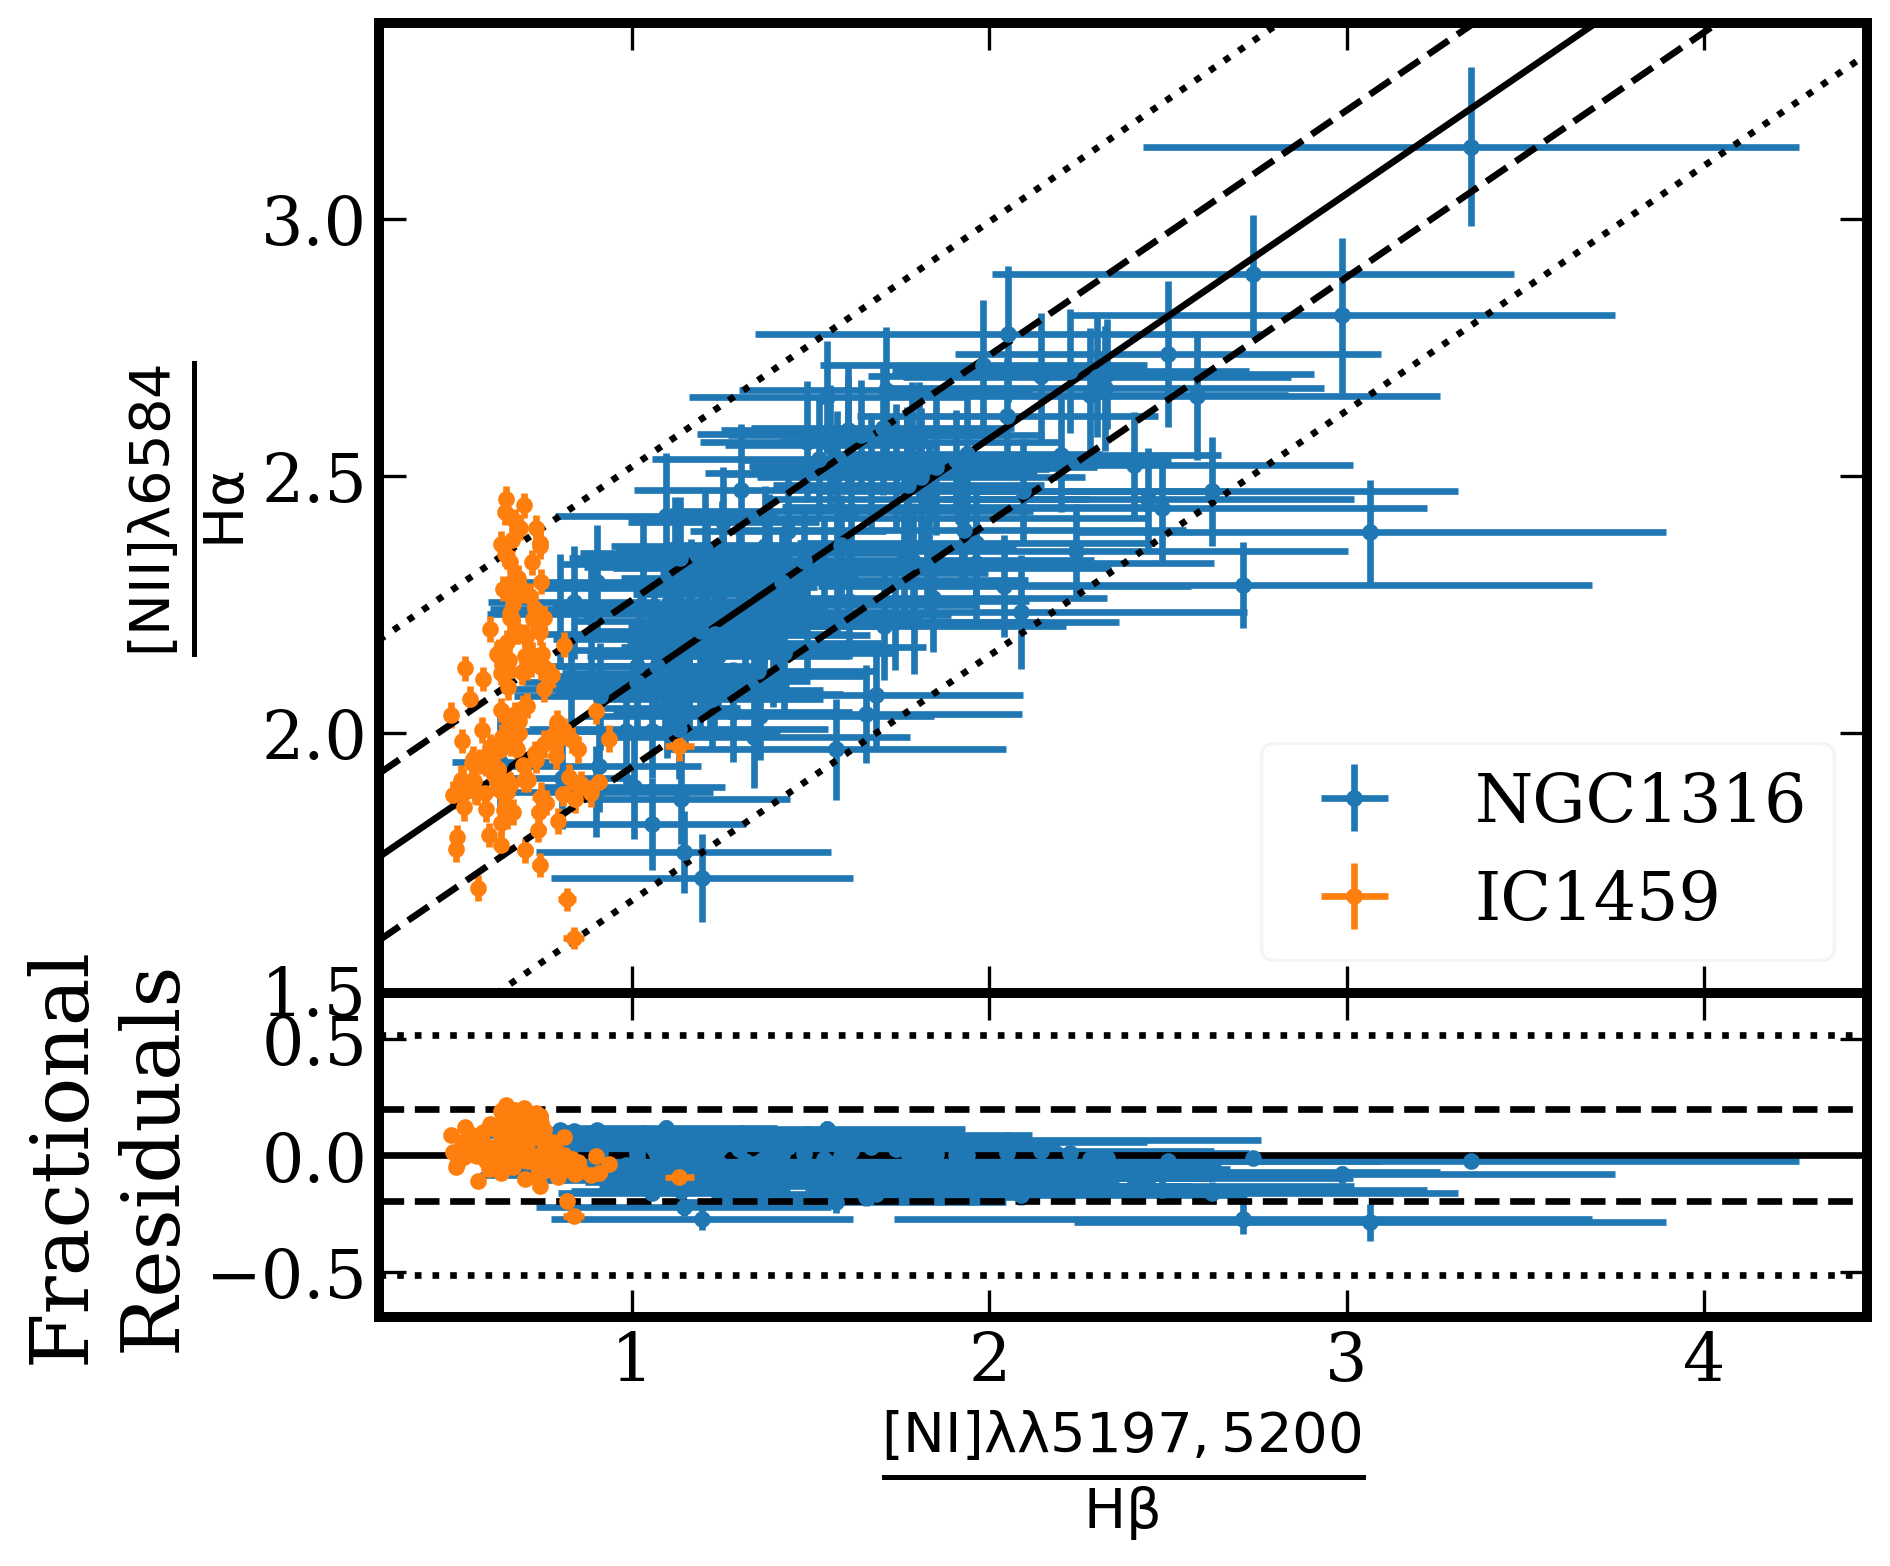
\includegraphics[width=\columnwidth]{ratio_fit.png}
  \caption[\bracket{\ion{N}{ii}}/H$\alpha$ vs.\
  \bracket{\ion{N}{i}}/H$\beta$]{Top: [\ion{N}{ii}]/H$\alpha$ vs.\
    [\ion{N}{i}]/H$\beta$ line ratios for the galaxies IC~1459 and
    NGC~1316, used to transform the classification boundaries of the
    classic BPT plot to the SAURON diagnostic plot. Bottom: Fractional
    residuals, defined as ([\ion{N}{ii}]/H$\alpha$ -
    best-fit)/[\ion{N}{i}]/H$\beta$. {\bf (Why do you divide by
      [\ion{N}{i}]/H$\beta$ rather than by [\ion{N}{ii}]/H$\alpha$?
      Change?)}  The solid lines show the best-fitting
    Eq.~\ref{eq:N_dec}, while the dashed and dotted lines show
    respectively the $68$ and $99\%$ probability contours. {\bf (The
      bottom y-axis label should be ``Fractional residual''.)}}
  \label{fig:ratio_relation}
\end{figure}

\begin{figure}
  \includegraphics[width=\columnwidth]{EQw_fit.png}
  \caption[EW(H$\alpha$) vs.\ EW(H$\beta$)]{As
    Fig.~\ref{fig:ratio_relation}, but for EW(H$\alpha$) vs.\
    EW(H$\beta$). {\bf (The bottom y-axis label should be ``Fractional
      residual''.)}}
  \label{fig:EqW_relation}
\end{figure}

% \begin{landscape}
\section{Maps}
\label{sec:maps}

Here we present the spatially-resolved maps of our Southern Sample
galaxies, one map for each of the parameters measured or fitted to the
IFS datacubes with the methods described in
Section~\ref{sec:analysis}. Each galaxy is presented in turn.

\begin{figure*}
  \centering
  % \includegraphics[width=\textwidth]{eso443-g024.png}
  \caption{Spatially-resolved map of all the parameters derived from
    the VIMOS observations of ESO~443-G24. Each parameter is indicated
    in the top-left corner of each panel, and the colour scale limits
    are listed in the bottom-right corner of each panel. {\bf (Why are
      these not perfect fits to the bottom-right corners? Fix?)} The
    surface brightness (isophotes) are overlaid as black contours in
    all the maps, while the \ce{^{12}CO(2-1)} contours from ALMA are
    overlaid in \removed{white} \added{cyan} {\bf (Pale blue or 
    turquoise? Correct.)} and the
    radio continuum contours from the VLA are overlaid in green. The
    radio band displayed depends on the data and angular resolution
    available \citep[see][]{ruffa2019, ruffa2020}. {\bf
      (``Metalicity'' should be ``Metallicity''. Also explain the
      meaning of the pale and dark greys bins.)}}
      % Preferable to rotate the colour table by $180$ deg, to match
      % the colour to the sense of the limits indicated in the
      % bottom-right corner of each plot?
  \label{fig:eso443}
\end{figure*}

\begin{figure*}
  \centering
  % \includegraphics[width=\textwidth]{ic1459.png}
  \caption{As Fig.\,\ref{fig:eso443}, but for IC\,1459 and derived
    from MUSE observations.}
  \label{fig:ic1459}
\end{figure*}

\begin{figure*}
  \centering
  % \includegraphics[width=\textwidth]{ic1531.png}
  \caption{As Fig.\,\ref{fig:eso443}, but for IC\,1531.}
  \label{fig:ic1531}
\end{figure*}

\begin{figure*}
  \centering
  % \includegraphics[width=\textwidth]{ic4296.png}
  \caption{As Fig.\,\ref{fig:eso443}, but for IC\,4296 and derived
    from MUSE observations.}
  \label{fig:ic4296}
\end{figure*}

\begin{figure*}
  \centering
  % \includegraphics[width=\textwidth]{ngc0612.png}
  \caption{As Fig.\,\ref{fig:eso443}, but for NGC\,612.}
  \label{fig:ngc612}
\end{figure*}

\begin{figure*}
  \centering
  % \includegraphics[width=\textwidth]{ngc1316.png}
  \caption{As Fig.\,\ref{fig:eso443}, but for NGC\,1316 and derived
    from MUSE observations.}
  \label{fig:ngc1316}
\end{figure*}

\begin{figure*}
  \centering
  % \includegraphics[width=\textwidth]{ngc1399.png}
  \caption{As Fig.\,\ref{fig:eso443}, but for NGC\,1399 and derived
    from MUSE observations.}
  \label{fig:ngc1399}
\end{figure*}

\begin{figure*}
  \centering
  % \includegraphics[width=\textwidth]{ngc3100.png}
  \caption{As Fig.\,\ref{fig:eso443}, but for NGC\,3100.}
  \label{fig:ngc3100}
\end{figure*}

\begin{figure*}
  \centering
  % \includegraphics[width=\textwidth]{ngc3557.png}
  \caption{As Fig.\,\ref{fig:eso443}, but for NGC\,3557.}
  \label{fig:ngc3557}
\end{figure*}

\begin{figure*}
  \centering
  % \includegraphics[width=\textwidth]{ngc7075.png}
  \caption{As Fig.\,\ref{fig:eso443}, but for NGC\,7075.}
  \label{fig:ngc7075}
\end{figure*}

\begin{figure*}
  \centering
  % \includegraphics[width=\textwidth]{pks0718-34.png}
  \caption{As Fig.\,\ref{fig:eso443}, but for NGC\,718-34.}
  \label{fig:pks718}
\end{figure*}

% \end{landscape}
% \clearpage

%%%%%%%%%%%%%%%%%%%%%%%%%%%%%%%%%%%%%%%%%%%%%%%%%%

% Don't change these lines
\bsp	% typesetting comment
\label{lastpage}
\end{document}

% End of mnras_template.tex
